%\chapter{Immersive Environments: XR}
\chapter{Question 3: Low-cost Dissemination of Spatial Computer Music}
\label{ch:xr-mus}

% \def\markchange{{\Huge\bf$\Rightarrow$}}
% \def\markchange{\marginpar[{\Huge\bf$\Rightarrow$}]{{\Huge\bf$\Leftarrow$}}}
% \markchange


Question \ref{ch:xr-mus} discusses how contemporary extended reality (XR) systems\footnote{XR includes VR, AR and MR. Virtual, augmented and mixed reality correspondingly.} can be exploited to enhance spatial music. Our main focus here will be to present how XR can be used as a dissemination tool, allowing the public greater access to this type of music. As a way to contrast the access issues surrounding XR, and in order to be thorough, we will also discuss some XR tools that are not low-cost or open-source - despite this being of primary interest.

% In chapter \ref{ch:spat-mus} we discussed tools for the creation of spatial music from a computer-music standpoint, with a focus on FOSS. Furthermore, we explored spatial instruments which facilitate the creation of such music works. Later, in chapter \ref{ch:spat-aud}, we focused on recording and reproduction means for spatial audio. In particular, we focused on ambisonic recording and reproduction tools, given their popularity in the open-source community interested in spatial audio. In this chapter, we would like to discuss how Extended Reality (XR) tools can also be used as for reproduction of spatial audio works. 

A large motivation for the creation and dissemination of spatial music stems from the growth of the XR industry in the last decade. Any complete discussion involving spatial music, therefore, should address how spatial music is being shaped by the development of these new tools. Over the years a number of scientists and companies have developed increasingly sophisticated XR systems in academic and commercial settings. Unfortunately, many of these XR system still remain too costly for most people. 

Our intention is to shed a light on various different types of XR technologies while focusing particular attention on technologies that allow for low-cost and open-source dissemination of spatial audio. We believe WebXR, in particular, is a powerful distribution tool which should be adopted by more artists working in the spatial audio domain. Online publishing is an important part of any artists work - allowing patrons to preview artists' works before committing to a live experience. WebXR provides musicians working with spatial music the opportunity to reach a wider audience, while preserving some of the depth that was carefully crafted into their music.

\section{What is XR?}

Before we dive into the role of WebXR in computer music, we should understand what exactly XR is. More specifically, for the purposes of our own work, we should understand what \textit{Virtual Reality} (VR) is. LaValle, defines VR in the introductory chapter of his free book "Virtual Reality" \cite{lavalle2016virtual} as a system containing four key elements:

\begin{enumerate}
    \item \textbf{Targeted behavior:} The organism is having an “experience” that was designed by the creator. Examples include flying, walking, exploring, watching a movie, and socializing with other organisms.
    \item \textbf{Organism:} This could be you, someone else, or even another life form such as a fruit fly, cockroach, fish, rodent, or monkey (scientists have used VR technology on all of these!).
    \item \textbf{Artificial sensory stimulation:} Through the power of engineering, one or more senses of the organism become co-opted, at least partly, and their ordinary inputs are replaced or enhanced by artificial stimulation.
    \item \textbf{Awareness}: While having the experience, the organism seems unaware of the interference, thereby being “fooled” into feeling present in a virtual world. This unawareness leads to a sense of presence in an altered or alternative world. It is accepted as being natural.
\end{enumerate}

Every XR experience is a \textit{perceptual illusion}. A programmer, or designer, has the task of creating an environment that attempts to fool another person's senses. This illusion can be aural, visual, or involve multiple senses - including smell, touch and taste. It should be noted, however, that this does not always mean the end goal is to make XR experiences as realistic as possible. Animations and \textit{lo-fi}\footnote{Low-fidelity.} graphic scenes are not only popular, but sometimes preferable to extremely realistic simulations.

In contrast to \textit{Mixed Reality} (MR) and \textit{Augmented Reality} (AR), VR experiences completely block out real-world sensory stimuli. Simple, overlay-style, applications are sometimes labeled as being \textit{AR experiences}. Meanwhile, MR is sometimes reserved for more sophisticated systems which require \textit{machine vision}. This, however, is not always the case. There are various MR systems that are marketed as being AR in nature\footnote{Most Apple products are marketed as AR, but behave much like MR systems.}. 

In a MR experience, an \textit{avatar} that is displayed in your \textit{Field of View} (FoV) might, for example, fall off a real table and respond to this event by holding its knee. This is not possible without a geometric representation of the space, which is obtained using some sort of light \textit{sensor}\footnote{Such as a camera.}. Machine vision, refers to the ability of a system to use camera data to detect characteristics of the real world. These include, but are not limited to, the positions of objects, or, a person's facial expressions.

In an AR experience, in contrast, we might see a simple display of time, temperature, coordinates, and humidity in the corner of one's glasses. This does not require any camera data to be generated, but instead uses other types of sensors. This information then gets automatically updated as the user moves from one location to the next. In these AR systems there is no link between the geometrical space, the objects inside it, and the system. Schmalstieg and Hollerer \cite{schmalstieg2016augmented} authored a comprehensive review of AR in their book: "Augmented reality: principles and practice". According to the authors AR implies the confluence of three elements:

\begin{enumerate}
    \item Combination of real and virtual worlds. 
    \item Interaction in real-time.
    \item Registration in 3D space. 
\end{enumerate}

The first and second part of this definition are quite clear: the system must bring together elements of the real and synthetically generated world, and, the system must respond to user interaction. The last element is defined by the authors as: 

\begin{quote}
    "...precise real-time alignment of corresponding virtual and real information. This mandate implies that the user of an AR display can at least exercise some sort of interactive viewpoint control, and the computer-generated augmentations in the display will remain registered to the referenced objects in the environment."
\end{quote}

In our previous example, the data from the real world is limited to: time, temperature, coordinates, and humidity. Therefore, according to Schmastieg and Hollerer, this does not qualify as AR. The MR example we provided earlier, however, would be called AR. This underlines the fact that companies and academics have different definitions of AR and MR, likely due to the infancy of the technology. 

Milgram and Kishino described in 1994 a continuum which can help categorize different XR experiences \cite{schmalstieg2016augmented}. Figure \ref{fig:continuum} shows this spectrum. The term AR here, refers to systems that are more real than virtual. \textit{Augmented virtuality}, refers to systems that are more virtual than real. For example, we can imagine computer generated worlds where avatars faces are real, but the rest of the environment is digital.

\begin{figure}[ht!]%force figure here, top, strict
\centering
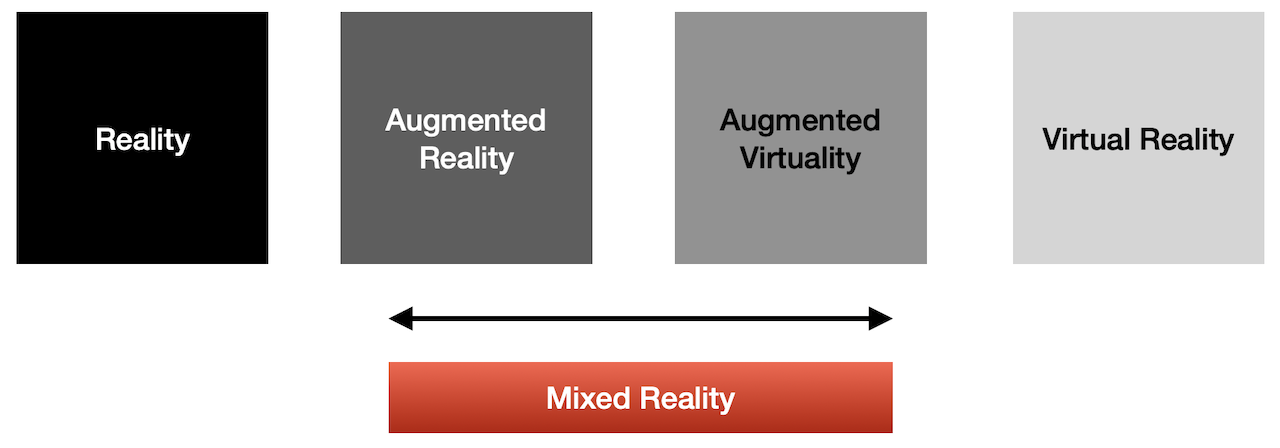
\includegraphics[width=0.7\textwidth]{img/continuum.png} 
%\captionsetup{justification=centering}
\caption{Milgram and Kishino Continuum}
% author: gabriel zalles ballivian (created using Apple Pages)
% public domain
\label{fig:continuum}
\end{figure}

Much like other authors in the field, if necessary, we will simply use the term AR in this text to avoid confusion. MR will be included in AR; we make no distinction between the two\footnote{It appears that MR is most prominent in industry products, however, fewer academic authors use this label.}. As new systems emerge, it is possible we will see even more types of "reality" emerge both in the academic and commercial sector. The lines are not always clear, especially when different senses are targeted by different systems than they were intended to. 

Consider a person seeing a VR experience with a VR display\footnote{Otherwise known as Head Mounted Displays (HMDs), these are "helmets" one wears which display images via screens mounted inside them. These will be covered in more detail later.} but listening to sounds from speakers, which are inadvertently being blended with real world sounds. The confluence of synthetic and real stimuli in the auditory domain point towards an AR experience. However, what if the real world sounds are not intended to be there? Is one of their senses in AR, and another sense in VR? If the real world sounds subside, does that change how we label the experience? 

\section{History of XR}

Much, much before the first ever "real" VR experience was ever developed, pioneering painters, from as early as the 15th century, were already working on the concept of depth perception and optical perspective. Today we take for granted the idea that 2D representations of 3D space contain any dimensionality, but before the establishment of cameras, this was a feature which had to be creatively articulated by artists. The idea of a \textit{vanishing point}, the point at which receding parallel lines viewed in perspective appear to converge, shaped an entire generation of painters. Figure \ref{fig:san-pedro} shows Pietro Perugino's use of perspective in the "Entrega de las Llaves a San Pedro" fresco at the Sistine Chapel (1481–82).

\begin{figure}[!htb]
\minipage{0.5\textwidth}
  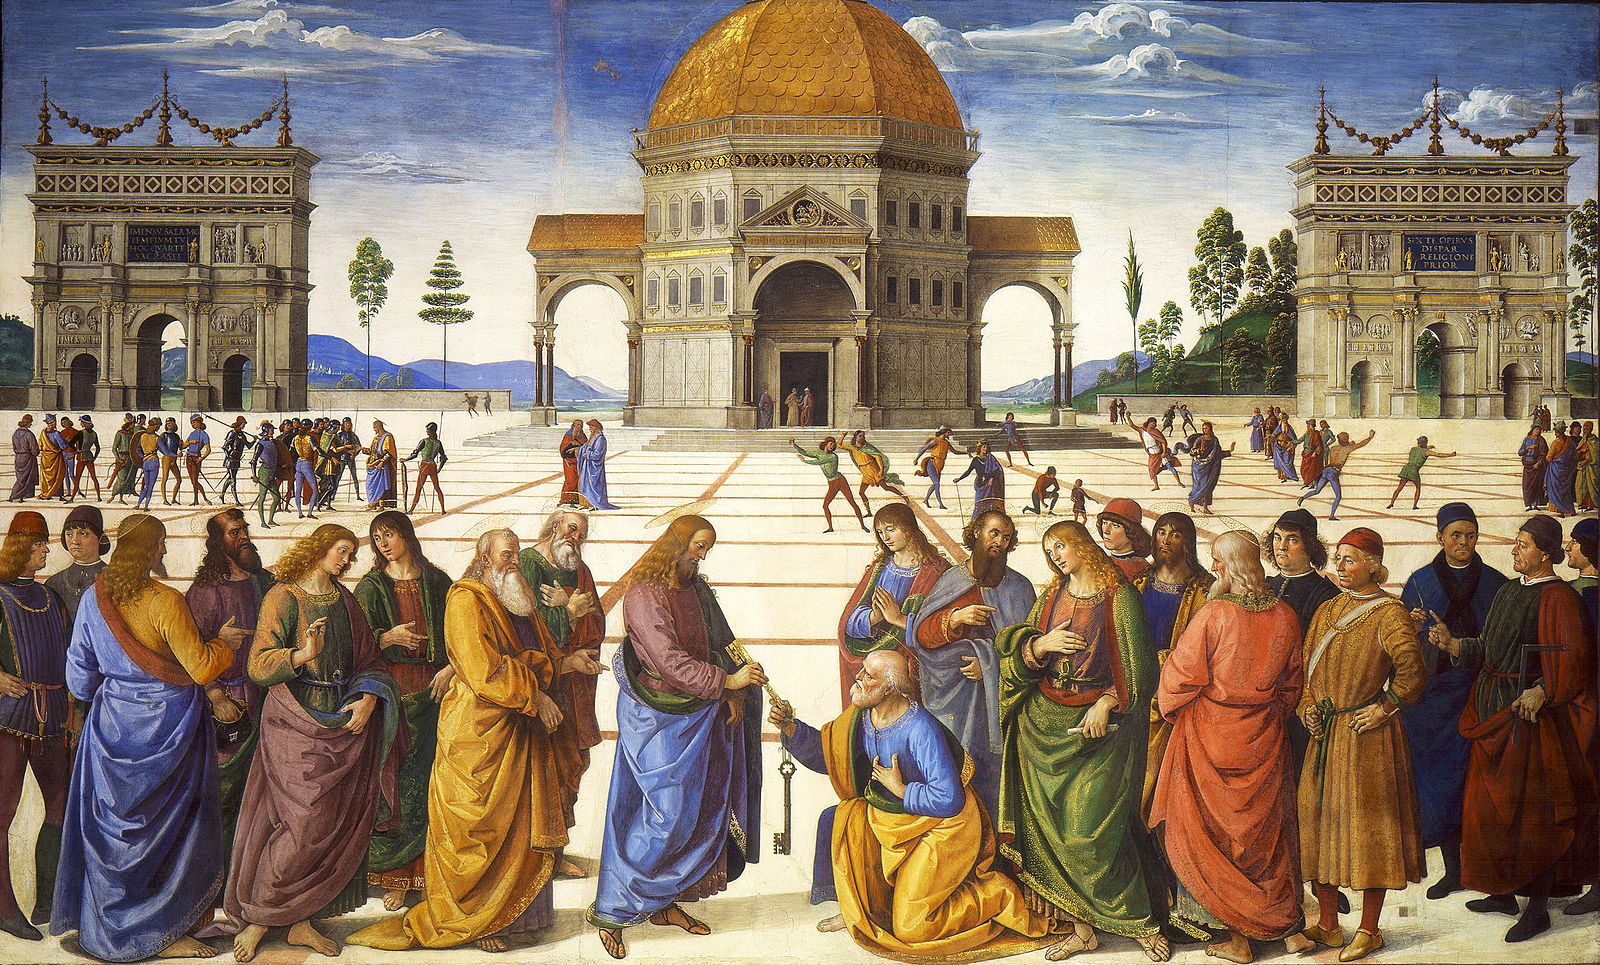
\includegraphics[width=\linewidth]{img/perugino.jpg}
  \caption{Vanishing Point Painting \cite{FileEntr24online}}\label{fig:san-pedro}
  % This work is in the public domain in its country of origin and other countries and areas where the copyright term is the author's life plus 100 years or fewer.
\endminipage\hfill
\minipage{0.5\textwidth}
  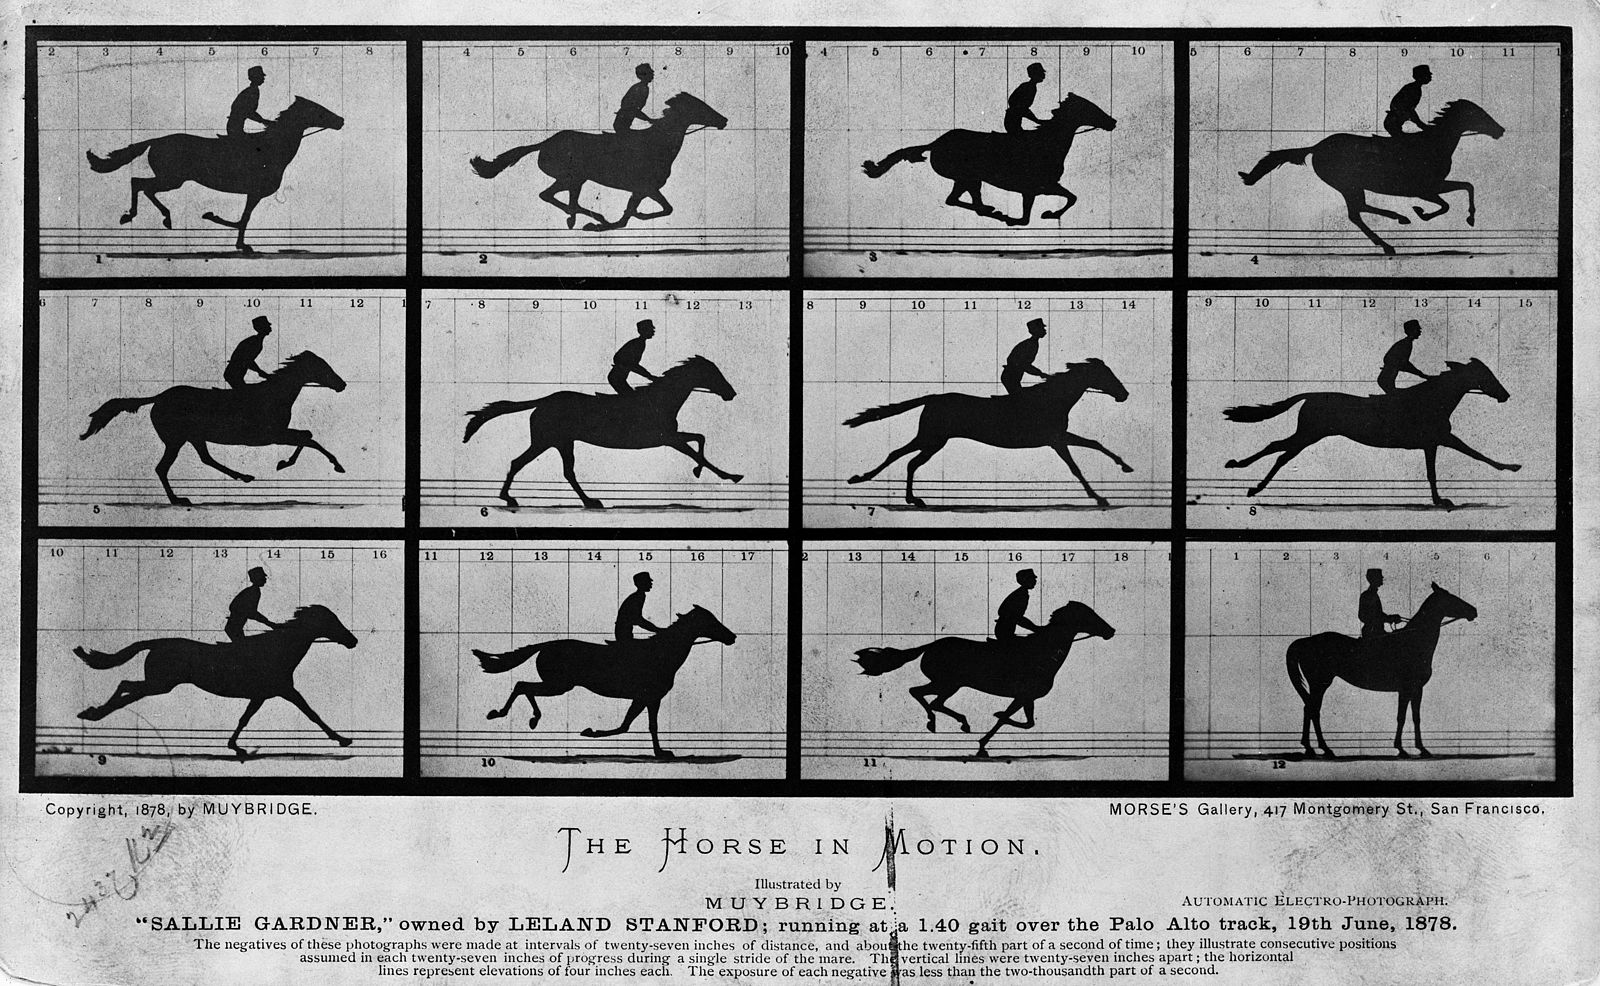
\includegraphics[width=\linewidth]{img/horse-in-mot.jpg}
  \caption{The Horse in Motion \cite{FileTheH64online}}\label{fig:horse-motion}
  % This work is in the public domain in the United States because it was published (or registered with the U.S. Copyright Office) before January 1, 1926.
\endminipage
\end{figure}

Much later, in the 19th century, the first \textit{stereoscope} was invented by Charles Wheatstone \cite{hemstrom2020comparison}. A stereoscope is a device in which a pair of slightly horizontally offset images of the same scene are presented to each eye, in order to provide additional depth perception. This exploits the fact that our visual system is always integrating two separate images, offset horizontally by the \textit{inter-ocular} distance, in normal viewing conditions. A picture of this device can be seen in Figure \ref{img:stereoscope}. By the 1930s, a portable version of a stereoscope called the \textit{ViewMaster} became commercially successful. The toy allowed people to switch images and see immersive photographs of places around the world. Some of the innovations of the stereoscope were the increased FoV and blocking of distracting boundary stimulus resulting in increased immersion. The ViewMaster, and other similar products, can seen as an early precursor to today's \textit{Head Mounted Displays} (HMDs), commonly used in VR experiences. 

\begin{figure}[ht!]%force figure here, top, strict
\centering
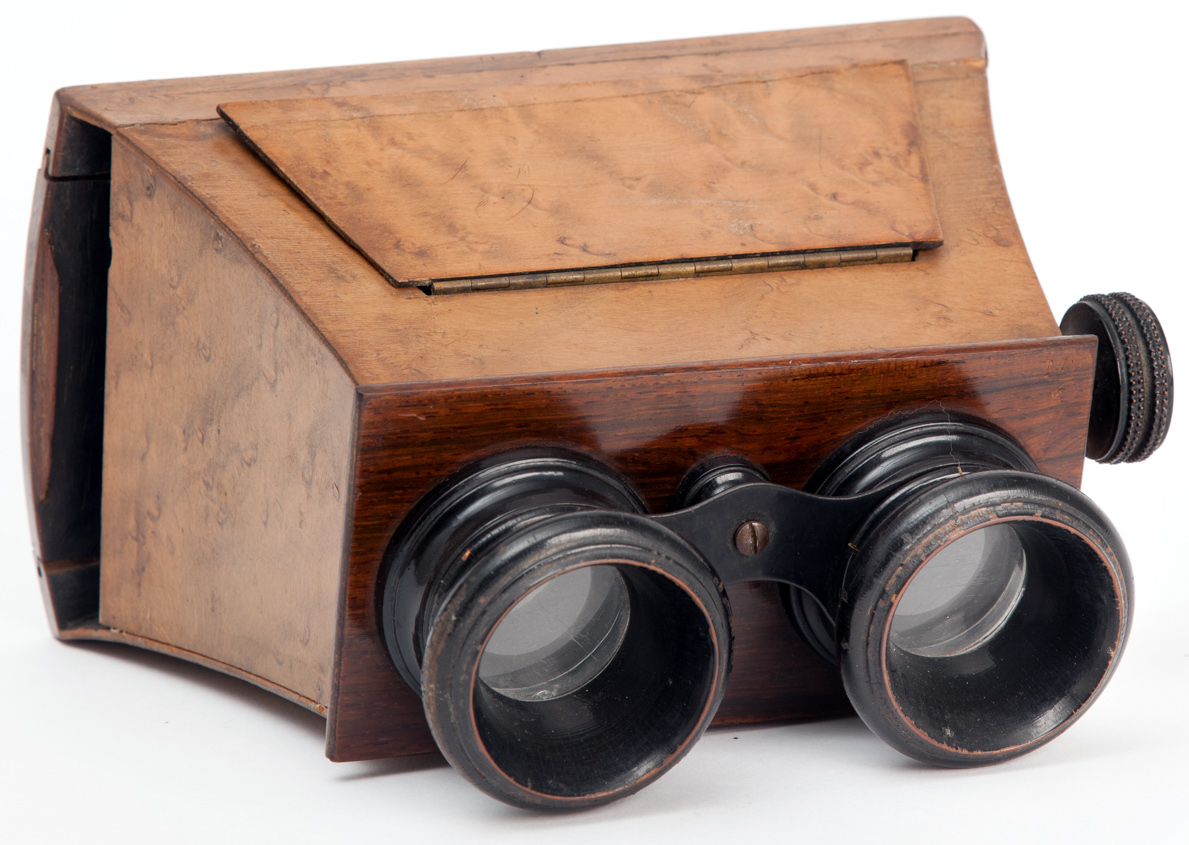
\includegraphics[width=0.4\textwidth]{img/stereoscope.jpg} 
%\captionsetup{justification=centering}
\caption{Brewster-type\protect\footnotemark stereoscope, 1870 \cite{FileIGB032online}}
\label{img:stereoscope}
\end{figure}

\footnotetext{Sir David Brewster (11 December 1781 – 10 February 1868) was a Scottish scientist, inventor, author, and academic administrator.}

In 1878, a few years after Wheatstone's stereoscope, one of the first examples of of \textit{stroboscopic apparent motion} was created by Eadweard Muybridge\footnote{Muybridge was an English photographer important for his pioneering work in studies of photographic motion (9 April 1830 – 8 May 1904)}. This effect refers to the ability to generate apparent motion by flipping through a sequence of images at a fast rate. Figure \ref{fig:horse-motion} shows Muybridge's famous work: "The Horse in Motion", which depicts several frames of a running horse, as it seemingly moves across space. In order to capture this sequence, 24 separate cameras were required. These were triggered by the horse as it moved along a track using ropes, which the horse's legs pulled on when running. The cameras were offset equidistantly to capture movements in a synchronized fashion. In order to reproduce the images, a \textit{zoopraxiscope}, also an invention of Muybridge's, was employed. The \href{https://upload.wikimedia.org/wikipedia/commons/0/06/The_zoopraxiscope-Horse_galloping-Animated.gif}{zoopraxiscope} is a disc containing multiple image frames which can be used to project a moving image in a recirculating fashion \cite{lavalle2016virtual}. 

Another well-known method in film-making used to increase realism, invented around 1915 by Edwin S Porter\footnote{Edwin Stanton Porter (April 21, 1870 – April 30, 1941) was an American film pioneer, most famous as a producer, director, studio manager and cinematographer.}, is \textit{3D film-making}. Modern 3D movies are created using special camera lenses and subsequently viewed using \textit{polarized} light filters. These filters, at the subjects eyes level, allow certain frequencies of light to pass into one eye, while blocking others. While there is a single image on the screen, two different images are perceived by each eye, much like with the stereoscope. \textit{Stereopsis} is the formal term describing the process of integrating two overlapping visual fields to achieve depth perception. 3D movies are still in use today in some VR experiences. They can also be found in commercial movie theatres across the world. 

\begin{figure}[ht!]%force figure here, top, strict
\centering
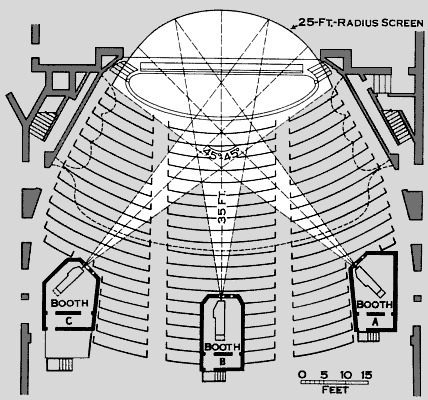
\includegraphics[width=0.5\textwidth]{img/cinerama.jpg} 
%\captionsetup{justification=centering}
\caption{Cinerama Diagram \cite{FileHowC90online}}
%public domain image
\label{img:cinerama}
\end{figure}

A different technique used to improve the sense of realism in movie systems involves increasing the FoV by using a wider screen that surrounds the viewer, accounting for viewers' peripheral vision. The \textit{Cinerama}, from the 1950s, is an example of such a system. It used three projectors to extend the FoV and projected the image upon a concave surface for a richer viewing experience. It was created in the 1950s, and can be seen as a precursor to the curved UltraWide LED (\textit{Light-Emitting Diode}) monitors popular today. 

A few years later, in 1957, Morton Heilig introduced the \textit{Sensorama}, which combined: motion pictures, stereo sound, vibration, wind, and even smells, in a personalized stereoscopic \textit{multi-modal} experience. The device resembles an arcade machine with an enclosure surrounding the subject's head, in order to reduce distractions. Unfortunately, the Sensorama had a fixed perspective, which meant the user was limited to a single orientation. It was also very large and expensive, which ultimately led to its downfall. Figures \ref{img:cinerama} and \ref{img:sensorama} depict the Cinerama and Sensorama respectively.

\begin{figure}[ht!]%force figure here, top, strict
\centering
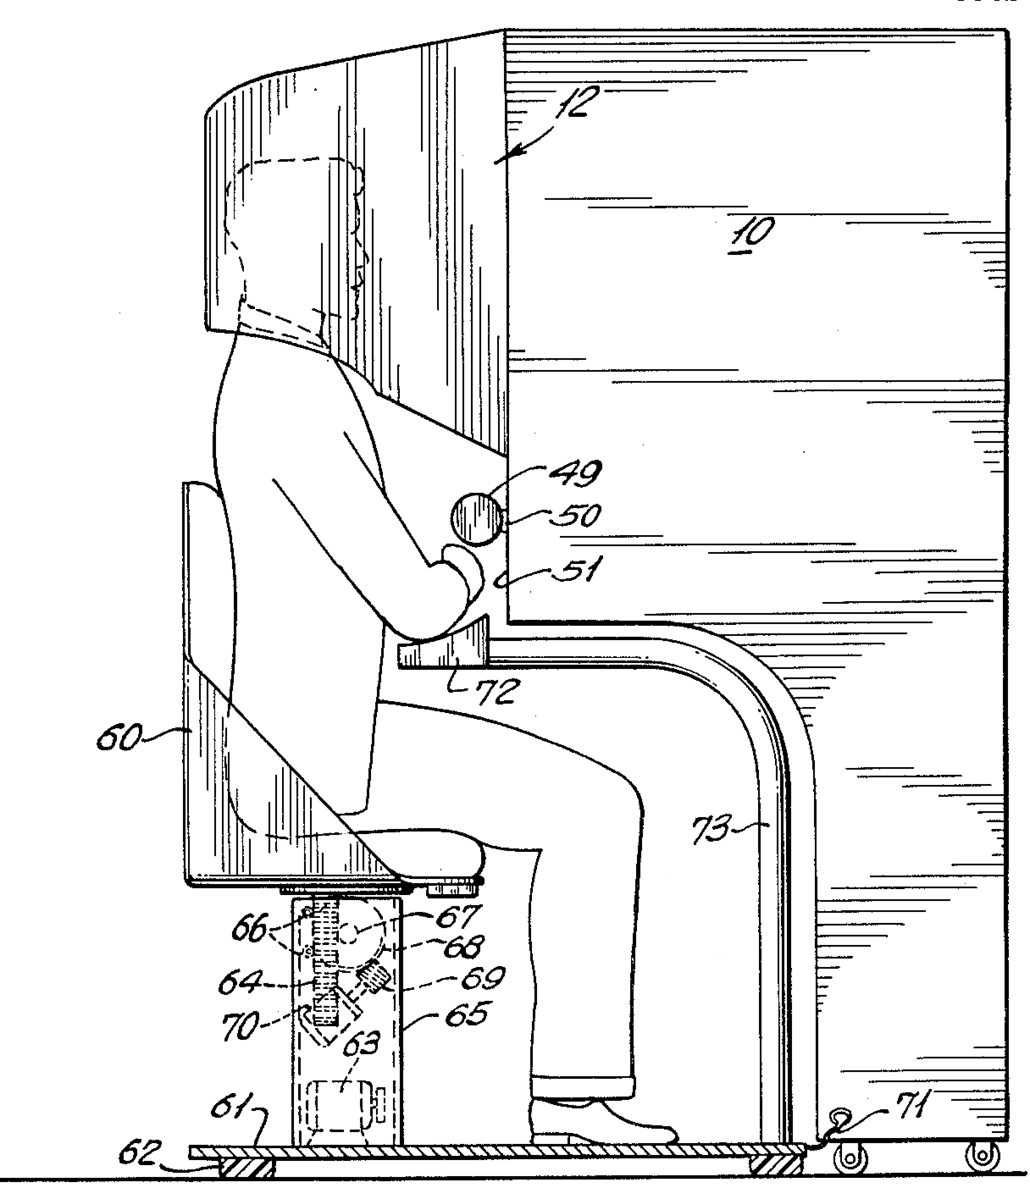
\includegraphics[width=0.4\textwidth]{img/sensorama.png} 
%\captionsetup{justification=centering}
\caption{Sensorama Patent Figure \cite{FileSens36online}}
%public domain image
\label{img:sensorama}
\end{figure}

Then, in 1965, a major step would be taken towards the realization of VR. That year, Ivan Sutherland\footnote{Ivan Sutherland (born May 16, 1938) is an American computer scientist and Internet pioneer, widely regarded as a pioneer of computer graphics.} introduced the concept of "The Ultimate Display", which he described as: "a room within which the computer can control the existence of matter." \cite{sutherland1965ultimate} A few years later, Sutherland and his team would build \textit{The Sword of Damocles}\footnote{You may find information regarding the myth \href{https://www.history.com/news/what-was-the-sword-of-damocles}{here}.}, regarded today as the first VR Head-Mounted Display (HMD). The display was a ceiling-suspended device capable of displaying simple wire-frame shapes according to the users' head movements \cite{hemstrom2020comparison}. This demonstrated for the first time in a virtual system the idea of the \textit{perception of stationarity}, which consists of making a static object appear to remain in its position while one moves their head. 

In the 1980s a number of advancements were made in the field, mainly by government agencies:

\begin{enumerate}
    \item In 1982, an advanced flight simulator called the \textit{Visually Coupled Airborne Systems Simulator} (VCASS) was created by the US Air-force Medical Research Laboratory.
    \item In 1984, the \textit{Virtual Visual Environment Display} (VIVED) was developed by the NASA Ames research center. 
    \item In the late 1980s, the term "Virtual Reality" was coined by Jaron Lanier, founder of the Visual Programming Lab (VPL). VPL would go on to develop the \textit{DataGlove} and the \textit{EyePhone} HMD. "Although all normal vision is lost wearing a HMD, the data glove allows the user to hold up their gloved hand in front of their face and see a digital representation through a HMD." \cite{dixon2006history}
\end{enumerate}

\begin{figure}[!htb]
\minipage{0.5\textwidth}
  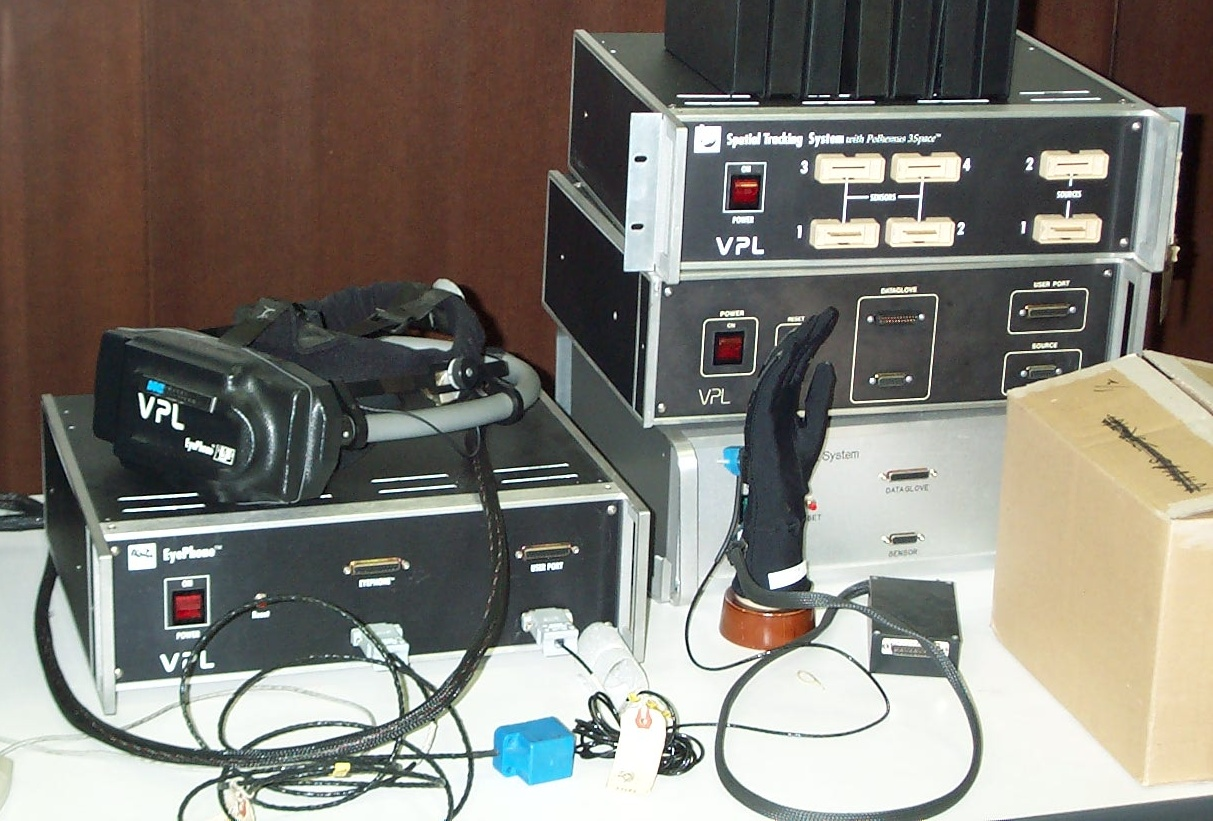
\includegraphics[width=\linewidth]{img/eyephone-dataglove.jpg}
  \caption{EyePhone HMD and DataGlove by VPL \cite{FileVPLE81online}}
  \label{fig:eyephone}
  %public domain
\endminipage\hfill
\minipage{0.5\textwidth}
  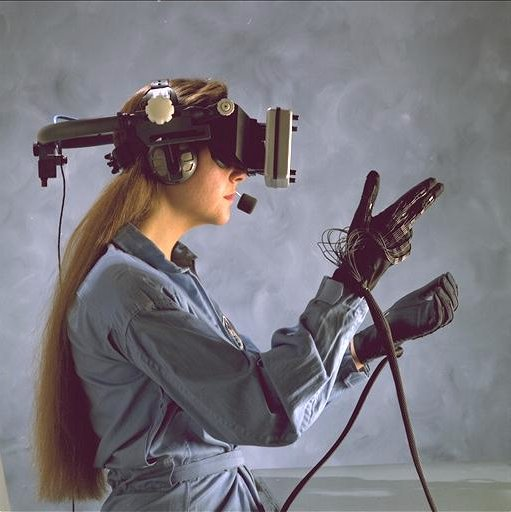
\includegraphics[width=\linewidth]{img/hmd-ames.jpg}
  \caption{HMD and Wired Gloves - Ames Research Center \cite{FileHead94online}}
  \label{fig:hmd-ames}
  %public domain
\endminipage
\end{figure}

Lanier went on to expand the DataGlove into a full body \textit{DataSuit}, capable of tracking users' different body joints. Using these suits, multiple users were able to interact inside a a virtual environment, and even change their physical appearance. In gaming, one's virtual representation is often called his or her \textit{avatar}.

A different approach, developed in the 90's, was the \textit{CAVE} (Cave Automatic Virtual Environment). This environment, developed in 1992 at the University of Illinois, uses a large number of projectors to, ideally, cover the entire surface of the room. Some CAVE systems also use 3D video in order to improve the depth perception of the image. The benefit of this approach is that the user does not need to wear any heavy equipment on their face which might restrict their ability to move. The downside is that such environments are often very costly to set-up given the large number of projectors needed to create the visual illusion. There are similar environments which use arrays of display panels in lieu of projectors to achieve higher visual fidelity.

\begin{figure}[ht!]%force figure here, top, strict
\centering
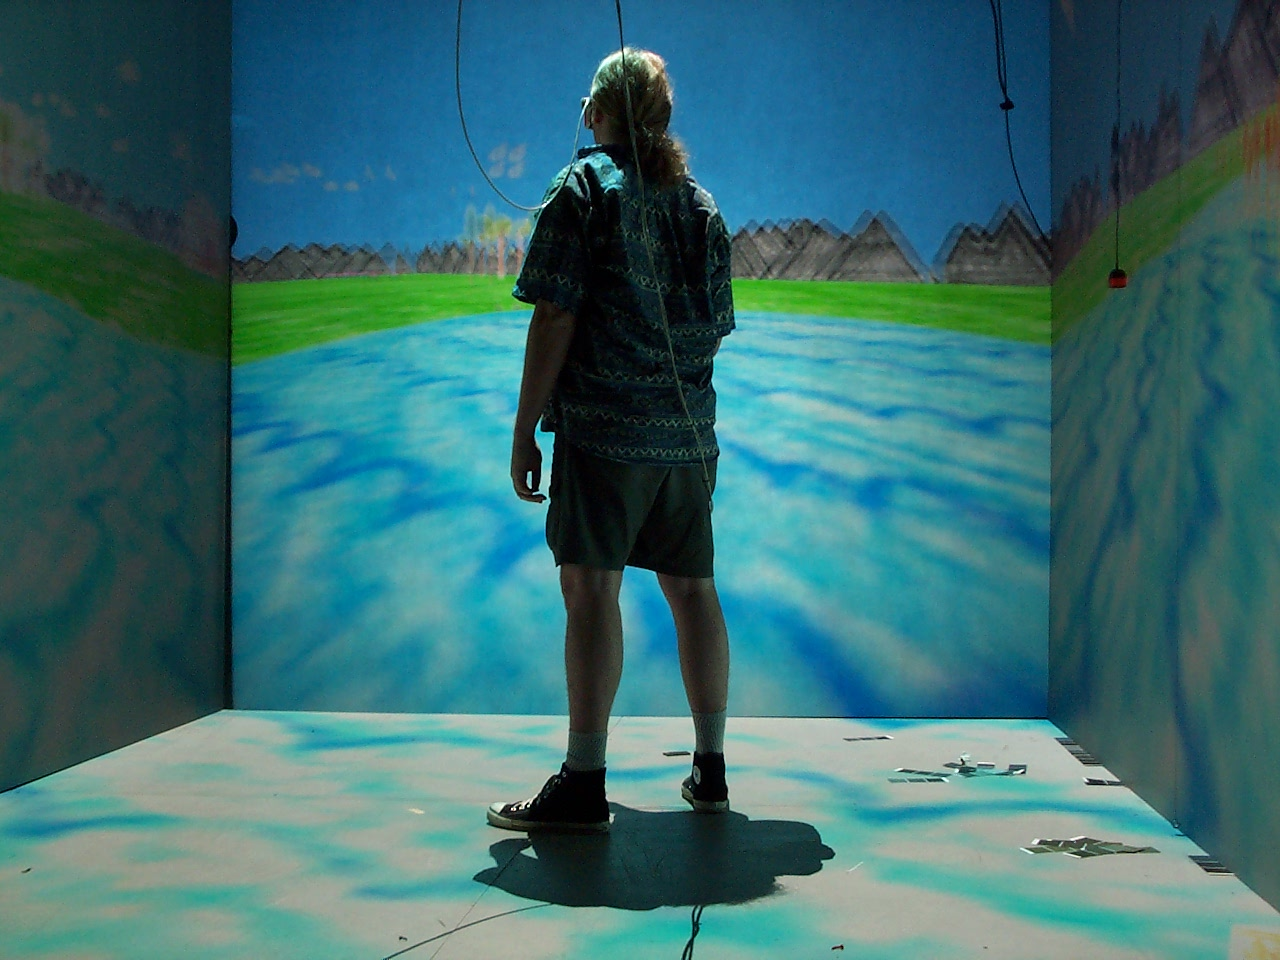
\includegraphics[width=0.6\textwidth]{img/cave.jpg} 
%\captionsetup{justification=centering}
\caption{CAVE \cite{FileCAVE71online}}
%public domain image
\label{img:cave}
\end{figure}

% \subsection{Head-Mounted Displays}

During this time there were also a small yet important number of artists who experimented with VR. Kazuhiko Hachiya created a two-person VR experience called \textit{Inter Discommunication Machine} in 1993, which switched one player's sight and sound for the others. The idea was to blur the lines between "you" and "me" \cite{dixon2006history} by switching sensory stimulation. At the Banff Centre, in Alberta, Canada, a number of VR projects were developed by a range of artists, all documented in Moser and McLeod's 1996 book "Immersed in Technology". Dixon \cite{dixon2006history} describes some of these projects in more detail. 

\section{Contemporary XR Techniques}

\subsection{Hardware}

\subsubsection{Degrees of Freedom (DoF)}

Chapter 2 of LaValle's book \cite{lavalle2016virtual} provides us with an overview of hardware practices important to XR. An important distinction LaValle makes in regards to hardware, is control in either \textit{three degrees of freedom} (3DoF) or \textit{six degrees of freedom} (6DoF). An ordinary object moving and turning in 3D space has 6DoF. Three of its degrees of freedom correspond to its changing position in space. These \textit{translations} include: 

\begin{enumerate}
    \item Horizontal (side-to-side) or $y-axis$ motion.
    \item Vertical (up-down) or $z-axis$ motion.
    \item Distal (front-back) or $x-axis$ motion.
\end{enumerate}

The other three degrees of freedom include: roll, pitch and yaw, which correspond to rotations along the $x$, $y$ and $z$ axes\footnote{This is our preferred coordinate system, it should be noted that others exist.}. Sometimes the \textit{user} will be given only 3DoF, in which case this is normally in the form of rotation changes. This is generally the case when viewing 360\textdegree \ videos, for example: videos in which a scene is captured in every direction using spherical lenses or arrays of cameras. The person is able to experience all directions of the video, by moving their head, but, generally speaking, cannot change the point of capture. In other words, translations in space is restricted. In this case the \textit{tracking system} (ie. the sensors in the display) only provide 3DoF.

Some controllers, such as the Sony Playstation \textit{DualSense} controller, have only 3DoF, which means they can send rotational information but are not designed for translation tracking. Sony's VR ecosystem uses the \textit{Move Controller}, which has an LED that is tracked by a camera system, which, when paired with its internal sensors, allows 6DoF. Some HMDs offer 3DoF only, while others are paired with external sensors, which report the position of the HMD in space to the VR system. This is generally accomplished using external cameras which track lights on the HMD. Other, newer systems\footnote{For example the Oculus Quest.}, use internal cameras to perform this task. 

\begin{figure}[!htb]
\minipage{0.4\textwidth}
  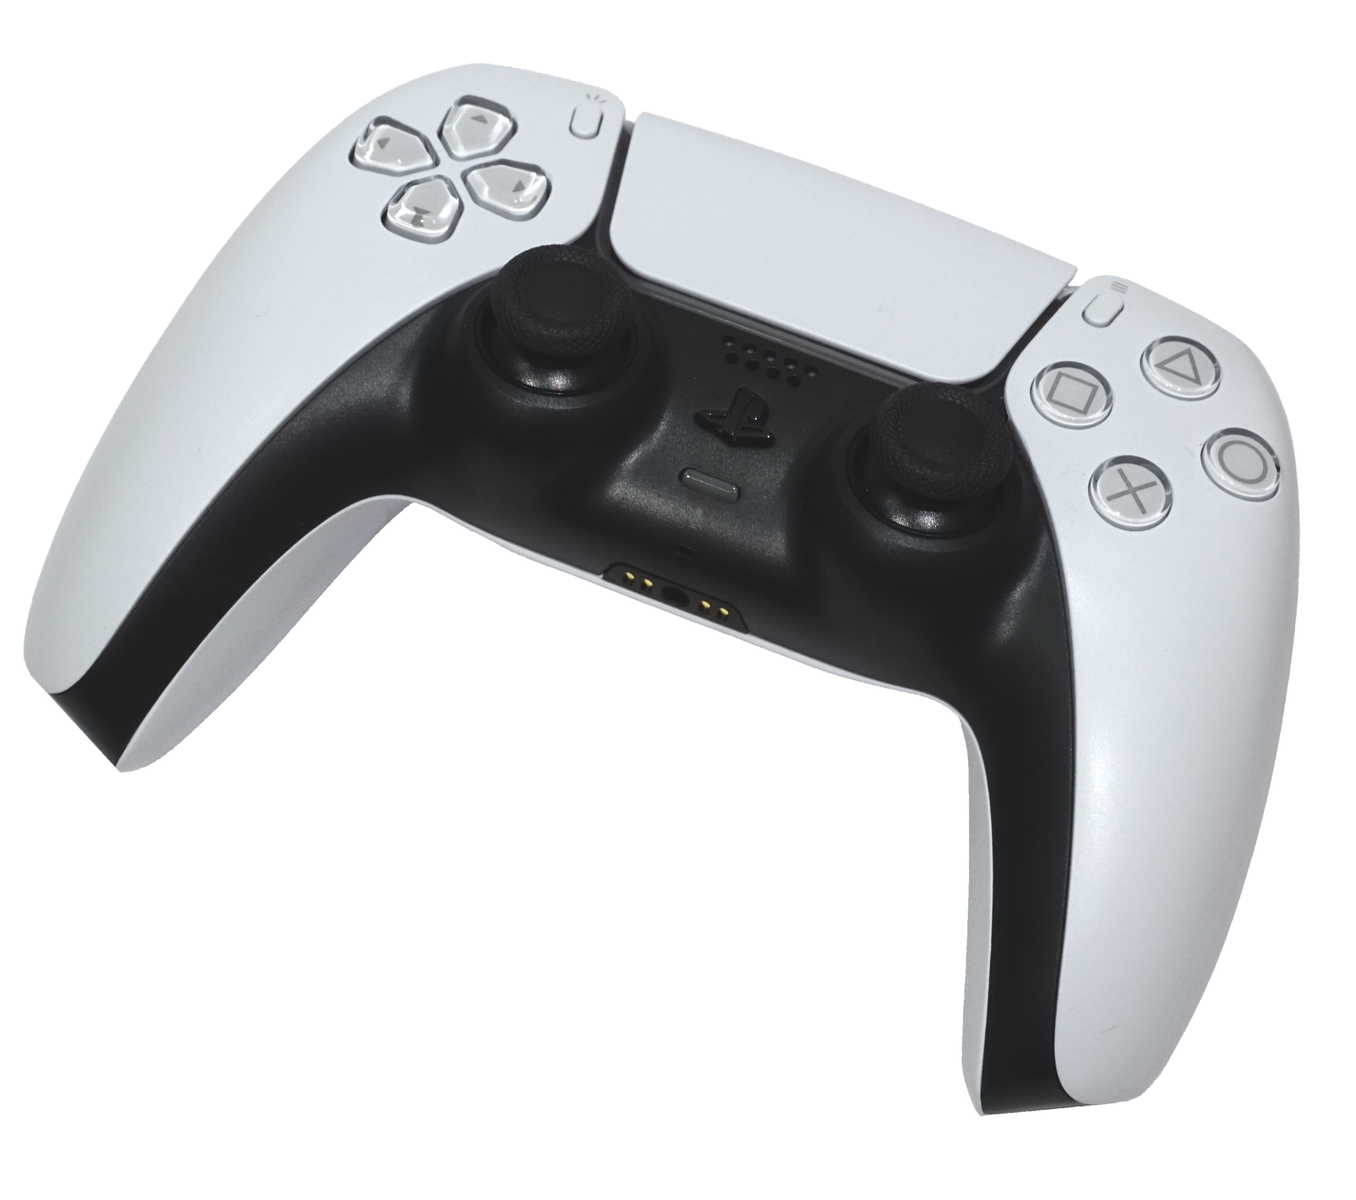
\includegraphics[width=\linewidth]{img/sony-dual.png}
  \caption{Sony DualSense Controller \cite{FilePlay5online}}\label{fig:sony-dual}
  % This file is licensed under the Creative Commons Attribution-Share Alike 4.0 International license.
\endminipage\hfill
\minipage{0.4\textwidth}
  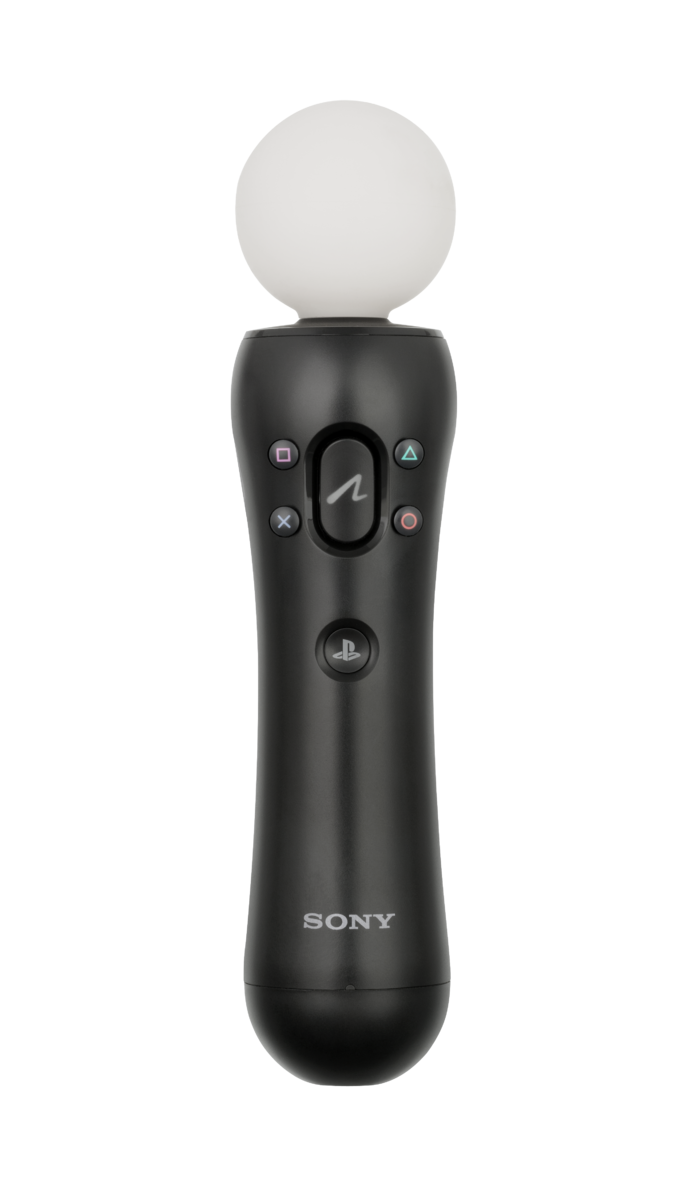
\includegraphics[width=\linewidth]{img/sony-move.png}
  \caption{Sony Move Controller \cite{FileSony89online}}\label{fig:sony-move}
  % public domain
\endminipage
\end{figure}

\subsubsection{World-fixed v. User-fixed}

Another important distinction we should make is between \textit{world-fixed} and \textit{user-fixed} systems. As we will see, user-fixed aural and visual displays offer a far more cost-effective and portable way of reproducing spatial audio and virtual scenes. World-fixed systems are less burdensome to the user, but often cost more to implement.

World-fixed systems refer to surround-sound systems, in the aural domain, and CAVE-like environments, in the visual domain. User-fixed systems refer contrastingly to binaural headphone systems and binocular HMDs, in the two respective domains. Both of these approaches to presenting XR experiences can be mixed. Each of them also have their own benefits and drawbacks. For sound systems, some of the key trade-offs between user and world fixed systems are:

\begin{enumerate}
    \item World-fixed systems require much more power (energy). Consider the power savings from binaural (headphone) reproduction versus surround-sound systems. 
    \item Headphones allow a sense of privacy, whereas surround-sound systems might disturb other people in your environment, or your neighbors. 
    \item User-fixed systems can be uncomfortable if used for long periods of time, since the user is required to wear heavy electronics on their head. 
    \item World-fixed systems might allow for multi-user experiences more seamlessly. However, there might be a noticeable drop-off in quality if users are outside the sweet-spot\footnote{Optimal viewing or listening position. HMDs and headphones do not have sweet spot problems.}. 
    \item Multi-user experiences are possible over headphones but require different sound processing for each user, which might prove computationally more expensive.
    \item Headphones are often much cheaper than surround-sound systems. 
\end{enumerate}

The trade-offs are quite similar in the visual domain. In world-fixed environments, it will only be necessary to modify the sound and visual scene according to users translational movements\footnote{If 6DoF is desired.}. Since they are already surrounded by audio-visual stimuli, natural rotational movements do not need to change anything in the environment. In contrast, user-fixed environments will need to adapt to user head rotations in order to create the illusion that they are inside an encompassing environment, which requires sophisticated graphics systems and a powerful computer.  

\subsubsection{VR Sickness}

An important problem to note here is poor updating of images in VR within user-fixed experiences. The slow frame-rate, or update speed, of these systems, can cause what is known as \textit{VR sickness}. This is caused by a mismatch in sensory information coming into the brain. This happens when one's \textit{vestibular} organs, used to maintain balance, are not in sync with one's visual organs. This is similar to the nauseating feeling we get when reading a book in a moving car. Over the years, GPUs\footnote{A Graphical Processing Units (GPU) is the part of the computer responsible for calculating and displaying images.} have become increasingly powerful, and, as a result, it is possible now to update images on HMDs quickly enough that VR sickness is eliminated\footnote{The amount of sensitivity to VR sickness is different from person to person, but, generally speaking, these systems work well enough now that they are mass produced and sold worldwide.}. CAVE-like environments do not suffer from this problem, however, much like in surround-sound systems, there is an optimal viewing area beyond which the image will not be of good enough quality. Ideally, in user-fixed systems, the frame rate is at least 90Hz, meaning there are 90 \textit{frames} per second. This number has become standard in the VR industry, since it seems to be the smallest frame-rate at which VR sickness is reduced to tolerable levels. 

\todo[inline]{Closed-loop vs. Open-loop}

\subsubsection{Dissecting XR Systems}

With the increasing pace of technological development, it can sometimes be difficult to categorize different systems and understand their relationship to the XR ecosystem. It is useful, in this context, to be able to dissect XR into its component part. Every XR systems can be divided into three primary parts \cite{lavalle2016virtual}:

\begin{enumerate}
    \item \textbf{Displays (output):} devices that stimulate your senses. %ch 4 and 5
    \item \textbf{Sensors (input):} devices that receive and interpret information from the real world. %ch 9
    \item \textbf{Computers:} devices which process inputs and outputs.
\end{enumerate}

% In the next few paragraphs we will describe these parts in more detail. 

\paragraph{Displays}

Displays, in the context of XR systems, refers to anything that is used to stimulate one's senses. They are simply outputs. Optical displays include projectors, such as in a CAVE, or HMDs - the counterpart to projectors in a user-fixed format. HMDs can be broken down into two main categories: \textit{dedicated HMDs}, and \textit{mobile HMDs}. Dedicated HMDs refer to visual displays whose function is solely to generate XR experiences. Dedicated HMDs can be broken down into two categories: \textit{tethered} and \textit{un-tethered}. 

As the name suggest, tethered HMDs require a direction connection to a computer, which sends video and power to the user's display. In turn, the tethered HMD also sends sensor information back to the computer, in order to update the displays in a cyclical fashion. Un-tethered HMDs refer to devices which have internal batteries, and powerful on-board processing units, allowing them to remain disconnected from an external computer. The GPU and CPU internally process any information needed, and wireless communication is possible with controllers and the web. 

Mobile HMDs, refer to HMDs which are based on mobile devices (ie. cellphones). Mobile HMDs are generally more cost-effective. However, since dedicated un-tethered HMDs are designed solely for the purpose of generating XR content, their internal components make them better at this task than most mobile-based systems. They are also substantially larger than mobile phones, which means they can hold bigger batteries and more computing power. On the software side, mobile HMDs operate either via standalone apps or WebXR solutions, both of which we will discuss in more detail later. 

\begin{figure}[ht!]%force figure here, top, strict
\centering
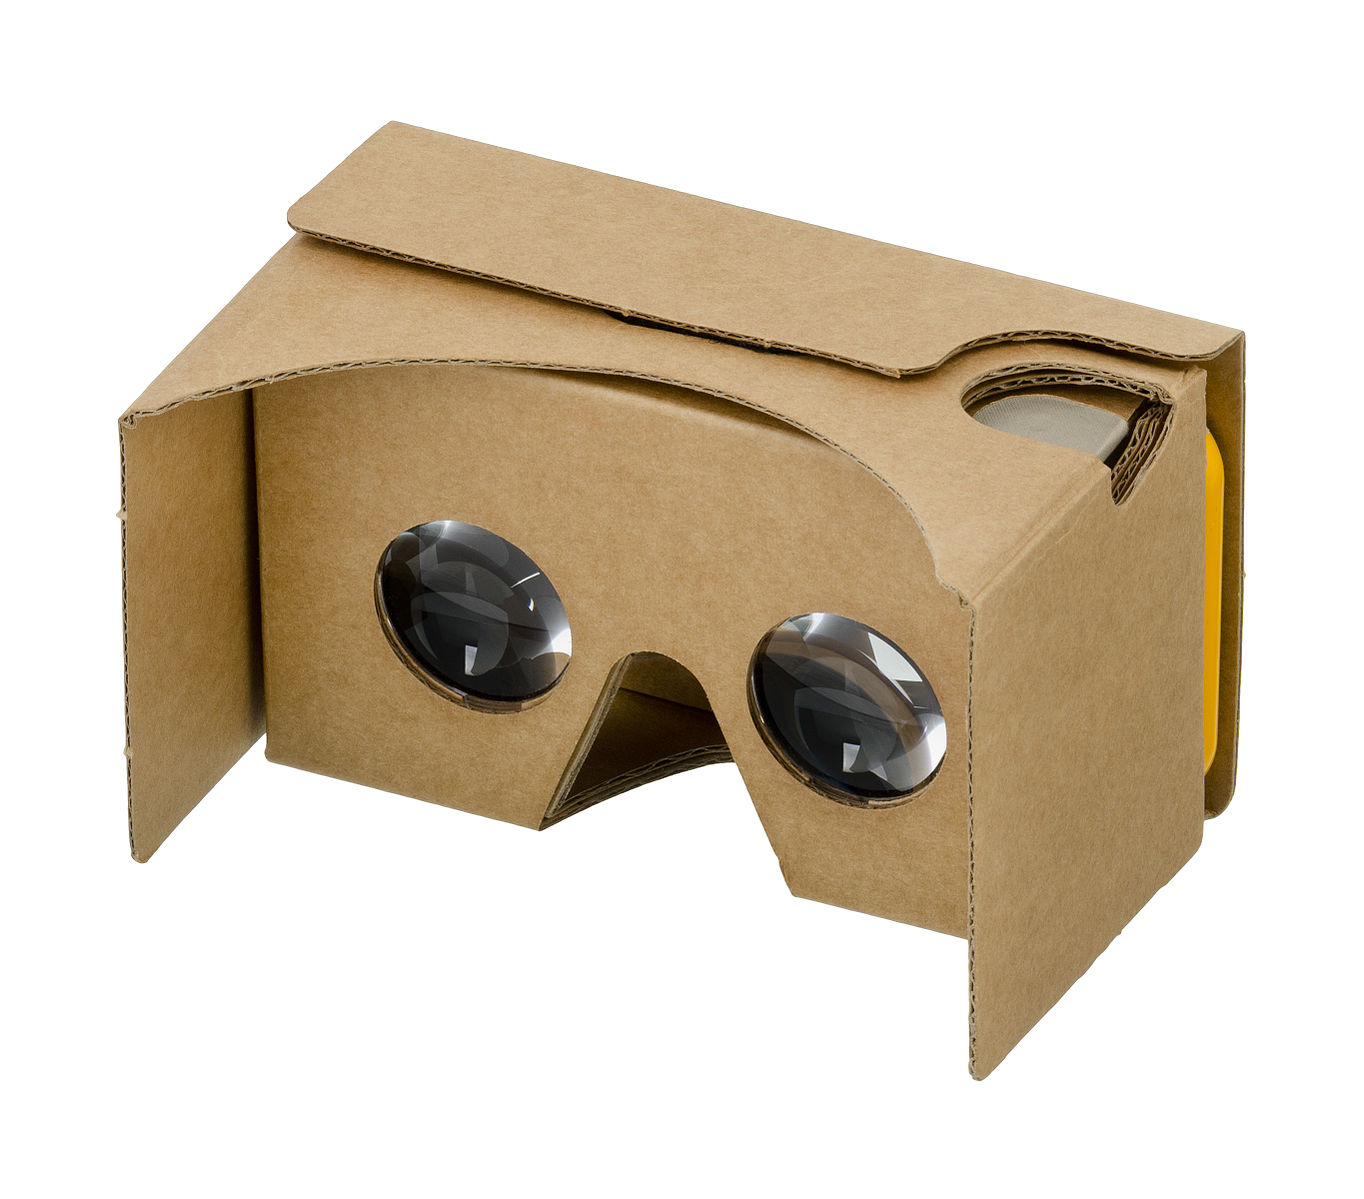
\includegraphics[width=0.5\textwidth]{img/cardboard.jpg} 
%\captionsetup{justification=centering}
\caption{Google Cardboard \cite{FileGoog63online}}
%public domain
\label{img:cardboard}
\end{figure}

An example of a mobile HMD is Google's \textit{Cardboard}, seen in Figure \ref{img:cardboard}. This simple HMD made out of cardboard can be used together with a smartphone to experience VR content with acceptable quality. It became popular in 2015, when the New York Times distributed the unfolded device to subscribers along with an app for VR journalism, focusing on the Syrian refugee crisis\footnote{The name of the aforementioned video is: "Displaced", by authors Ben C. Solomon and Imraan Ismail \cite{TheDispl63online}.}. Much like with other HMDs, two small magnifying lenses, usually \textit{Fresnel lenses}, are situated in front of the eyes. 

XR displays can also be found in the aural domain. These include surround-sound systems, headphones, or \textit{bone-conduction headphones}. Bone-conduction headphones send vibrations directly to the skull which is connected to our auditory system. There are also some XR HMDs which use small speakers near the ears to provide an auditory AR experience. Additionally, there are displays for our other senses. The most commonly encountered display for \textit{haptic} feedback is vibration systems, which are used in controllers. 

AR HMDs offer another form of optical display. Rather than placing screens in front of the subjects eyes, these place transparent surfaces upon which light is emitted. This allows the user to see both the real world and additional objects the experience provides. Figure \ref{img:ar-glasses} shows a man wearing a pair of AR Glasses. 

\begin{figure}[ht!]%force figure here, top, strict
\centering
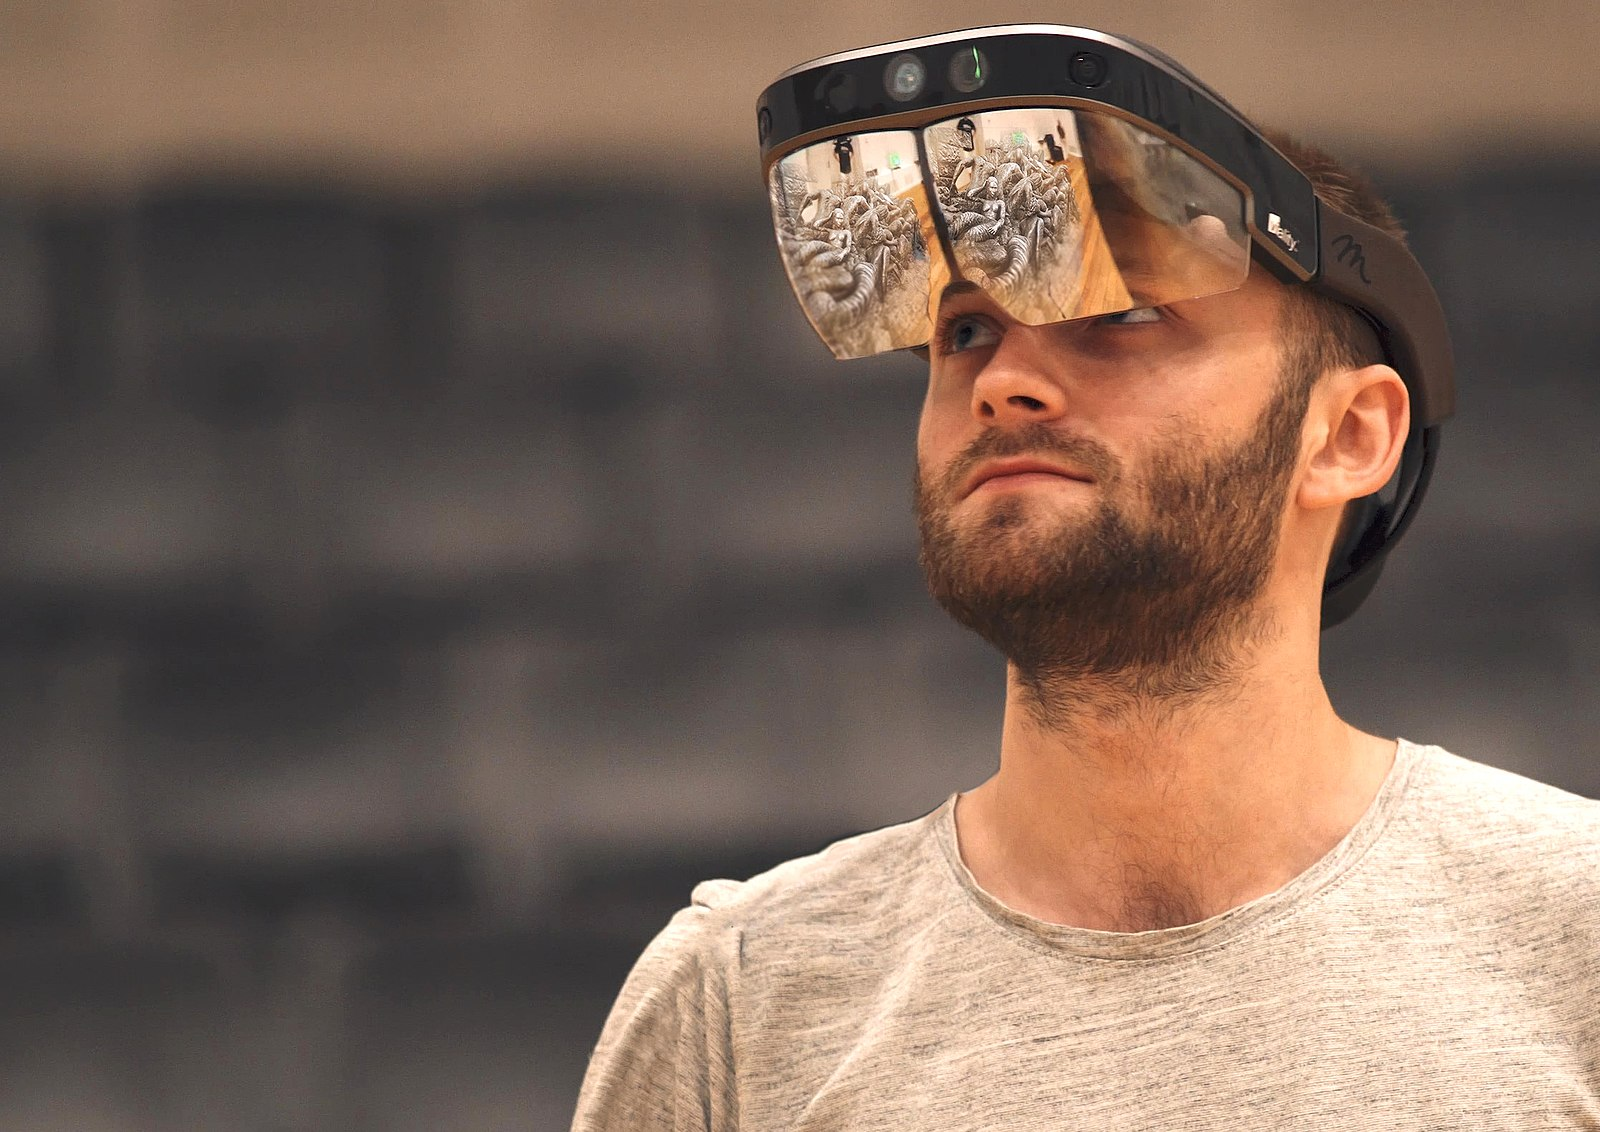
\includegraphics[width=0.6\textwidth]{img/ar-glasses.jpg} 
%\captionsetup{justification=centering}
\caption{Man Wearing AR Glasses \cite{FileWear23online}}
%Creative Commons Attribution-Share Alike 4.0 International license.
\label{img:ar-glasses}
\end{figure}

\paragraph{Sensors}

Sensors refer to inputs the computer-system will receive in order to accurately render the scene for the user. The most salient information needed for XR applications employing HMDs is gyroscopic data. Gyroscope are embedded in most of today's cellphones, and all dedicated HMDs. These report the orientation of the user's head back to the rendering software. Gyroscopes are also sometimes found inside controllers, such as inside the Sony Move Controller we showed earlier. 

The number of controllers, or sensing systems, available today is exceedingly large. It would be impossible to list them all here. Instead we provide a short list of some additional popular sensors: 

\begin{enumerate}
    \item \textbf{The Leap Motion Controller}: is an infrared camera system used to detect and track human hands, including independent joint movements and fingers. It can be used in lieu of VR controllers.
    
    \item \textbf{Microsoft Kinect}: is a camera and \textit{infrared} sensor system capable to performing depth mapping, and track entire bodies. It can be used to track body orientation and movement of large appendages. This is accomplished by projecting infrared light unto surfaces and capturing the reflection. 
    
    \item \textbf{Game Controllers:} many people familiar with game controllers, such as those from Sony or Microsoft, prefer playing in VR using these standard controllers - over \textit{VR controllers} - even though some only provide 3DoF. An example of a game controller is the Sony DualSense Controller.
    
    \item \textbf{MOCAP}: a MOtion CAPture systems, is similar to a Kinect, but capable of tracking bodies in a larger area, and uses multiple camera angles. This means that subjects do not need to face any particular direction. In order to track limbs, special suits which reflective balls are worn by subjects. These are specialized systems, and tend to be more costly than mass produced video game devices. 
    \item \textbf{VR Controllers}: in addition to the Sony Move Controller there are various designs by Oculus\footnote{A Facebook subsidiary.} and \href{https://www.htc.com/us/}{HTC}. Some other HMDs, especially those for MR, use cameras to track fingers, much like a leap motion would. 
    
    \item \textbf{Facial Tracking}: this type of input is more common in AR applications. The technology allows detection of faces and analyzes facial expressions. Digital masks or filters can follow the movements of the face. 
\end{enumerate}

In addition to all these devices some people also opt to use a standard keyboard and mouse system for interacting in XR. There are also custom-made sensing devices out there created from prototyping parts which can communicate to the software via wireless protocols. Finally, there are various specialized controllers designed for specific tasks, such as controllers resembling plastic rifles, used in war games, for example.

\begin{figure}[ht!]%force figure here, top, strict
\centering
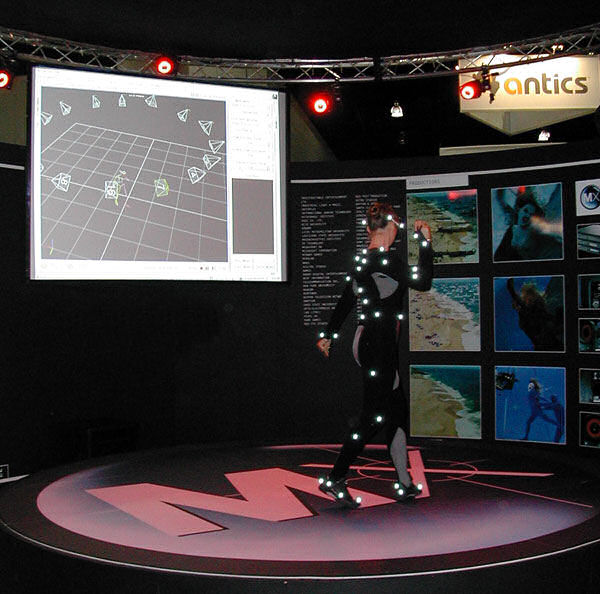
\includegraphics[width=0.75\textwidth]{img/mocap.jpg} 
%\captionsetup{justification=centering}
\caption{MOCAP System \cite{FileMoti99online}}
%public domain
\label{img:mocap}
\end{figure}

One of the complications that can sometimes arise in sensor or controller design is the problem of \textit{registration} in VR. If the objects are not registered, because they are not tracked by the system, then the person has no way of locating the object in the real world. Some companies provide locators which allow users to register different objects in VR by attaching any 3D model they want to the object. For example, one can specify a real guitar is being used and attach the model of a guitar to the hands of the user - allowing them to find their guitar once inside VR. This is one of the advantages of AR over VR: there is only partial \textit{occlusion}; as a result, subjects can easily locate the items they wish to interact with in the real world.

Certain successful designs exploit \textit{proprioception}, which is our sense of where our extremities are without having to see them. For example, with the aforementioned Kinect, we don't necessarily need to see a representation of our body in VR to know where our appendages are. We can easily perform any movements the system requires without directly needing to see them happen. In most cases, however, registration of sensors is preferable, as they give users direct feedback to confirm the actions they are undertaking. 

\paragraph{Computers}

Once all the inputs and outputs are known, it is the task of the computer to analyze incoming data and present stimuli to the user via various displays. The capabilities of the computer will determine how much data it can analyze and how much data it can return. As we have noted, some cellphones are able to generate virtual worlds, however, because these have less powerful computing hardware, the graphic scenes generally need to be simpler. 

Within the computing hardware, there are various sub-systems which work together to provide a smooth experience. The \textit{Graphical Processing Unit} (GPU), is responsible to \textit{rendering}\footnote{Calculating vertex, edge, and face positions, and subsequently displaying them. They also perform lighting and shadowing.} the graphical content. The \textit{Central Processing Unit} (CPU) is similar to the GPU, however, is not designed for graphics - instead it handles all the other calculations, commands and processed necessary. In some designs, a \textit{Micro-Controller Unit} (MCU) is also used to handle inputs and relay the information to the CPU, which may be tethered to or inside the HMD.

Some of the important factors to consider here are portability and also the ease of prototyping. When developers are creating these experiences, they need a way to quickly create environments and test them out. Wireless devices might prove more difficult to work with in this regard.  

\todo[inline]{display interface chips?}

\section{Software}

Generally speaking, today, there are three main platforms that are \textit{targeted} by game developers. For each of these different targets, there are associated software libraries that allow us to create content. \textit{Game engines} are the most powerful of these three platforms. These software environments are designed to facilitate the creation and customization of video games and XR experiences. Secondly, there are mobile apps, for which there exist various different \textit{Software Development Kits} (SDKs) with different flavors depending on the operating system of the mobile device. Finally, there is \textit{WebXR}. This corresponds to applications that run on the browser, be it via a mobile phone, HMD, or a traditional computer - with a mouse, keyboard and monitor. 

\subsection{Game Engines}
% Unity, Unreal, Godot, etc.

Game engines are software-development environments used to create video games or XR experiences. The core functionalities of these engines include:

\begin{enumerate}
    \item \textbf{3D graphics}: determines how objects are displayed on screen. It should, for example, consider vanishing point, occlusion and parallax. 
    \item \textbf{Physics engine}: determines how light scatters, objects move, and other attempts to simulate real world physical behaviors. 
    \item \textbf{Collision detection}: responsible for detecting contact between objects. 
    \item \textbf{Sound}: this might include spatial audio systems, which simulate 360\textdegree \ sound using \textit{binaural} filters.
    \item \textbf{Scripting}: the ability to customize behaviors based on developer needs. 
    \item \textbf{Animation}: importing objects with built in movement behaviors. For example, a model of a bird with its wings flapping.
\end{enumerate}

Today, the most popular game engine is likely \href{https://unity.com/}{Unity} which is cross-platform\footnote{Works with multiple operating systems, including Linux.} and allows \textit{building}, or targeting, a multitude of platforms, including: Mac, Windows, WebGL, iOS, and WebGL - to name a few. Unfortunately, the license is proprietary - however it does offer exclusive support for educational purposes, making it a useful tool for pedagogical purposes. Another game engine that is gaining popularity, due to its open source nature, is \href{https://godotengine.org/}{Godot}. However, it is not as well-featured as Unity, given that it is much younger. One final game engine we should mention is \href{https://www.unrealengine.com/en-US/}{Unreal} which is commercial in nature but whose \textit{source code} is available online. 

All of these game engines, as far as XR is concerned, are suited for creating content targeting HMDs, but world-fixed systems do not seem to be natively supported. Tredinnick et al. \cite{unicave2017} propose a plug-in for the game engine Unity, which allows one to use the software with "distributed immersive tiled or projection-based VR display systems", such as a CAVE. It is possible to use internal audio routing software to decode ambisonics from other software, but perhaps one could also develop a plug-in which allowed for this natively. 

\subsection{Mobile XR}

Mobile XR SDKs are used to develop apps and experiences which can be downloaded and run on cellphones. Sometimes these experiences come in the form of 360\textdegree \ videos, other times the applications are graphical renderings of scenes composed in game engines. Various large technology companies, such as Google and Samsung, have created mobile XR development software. In the next few sections, we will explore some of these projects. It should be noted that, with the proliferation of standalone HMDs, mobile VR SDKs are beginning to lose support from these companies. We believe it is only a matter of time before most of these development platforms are entirely irrelevant in the VR ecosystem. Mobile AR SDKs are still being supported, and are finding new applications every day.

\subsubsection{Mobile VR}

Mobile VR SDKs are development kits used to create VR applications targeting mobile devices. The three most popular platform in this area are the: Google \textit{Cardboard}, Google \textit{Daydream}, and Samsung's \textit{Gear VR}. Each of these different platforms has different SDKs which allows users to create VR experiences for them. As we can see, all of these different platforms are proprietary and as a result there are limits to what developers can do with them. 

Unfortunately for consumers, over the last few years mobile VR SDKs have lost a lot of support\footnote{Time of writing 2021.}. This is due to the fact that both Google and Oculus\footnote{Gear VR was a collaboration between Samsung and Oculus.} have transitioned into selling standalone HMDs. Fortunately, Google still supports the Cardboard environment to create VR experiences. Since the Daydream project and Gear VR project are now both considered \textit{legacy}\footnote{Outdated systems, in computer science parlance.} systems, we will discuss a bit here only about the Cardboard environment. 

\paragraph{Cardboard SDK}

The recent releases of the Cardboard SDK by Google allow developers to target iOS and Android devices. One can also use the SDK inside Unity if desired. The SDK is licensed under \href{https://www.apache.org/licenses/LICENSE-2.0.html}{Apache License 2.0}. Given the simple nature of the Cardboard HMD, the \textit{Application Programming Interface} (API) only allows for monitoring the input of a single button. Naturally, the system internally perform motion tracking and stereoscopic rendering. Because of the interactive limitations of the system, most of the apps for this system are exploration or content viewing apps. One example of these is the \textit{Within VR} which features political, kids, and science 360\textdegree \ videos.

\subsubsection{Mobile AR}

Mobile XR comes in two types: \textit{native} and web-based applications. For example, within mobile VR, viewing a Youtube video that is \textit{streaming} from the browser is a web-based application. Meanwhile, with apps like \textit{Within VR}, the user downloads these videos in their entirety before viewing. This is a native application that does not rely on a browser of internet connection (once the video has been downloaded). 

Mobile AR also comes in these two styles: native and web-based. Since web-based applications will be discussed in more detail later, in this section we will only discuss software platforms used to develop native mobile AR applications. iOS and Android are the two most common OSs for mobile devices today, and both offer different SDKs to create AR applications. In the next few paragraphs we will discuss some of the features of the most popular SDKs for mobile AR applications. 

\paragraph{ARCore}

ARCore is an open-source Google project allowing one to create AR apps for Android or iOS. It can also integrate with Unity or Unreal. Its main features include motion tracking, environmental understanding and light estimation. One can also use the SDK for developping WebXR applications. There is also an Android \textit{Native Development Kit} (NDK) written in C. The following list describes in some more detail the features of this development library.

\begin{enumerate}
    \item \textbf{Motion tracking}: ARCore uses \textit{Simultaneous Localization And Mapping} (SLAM) to "understand where the phone is relative to the world around it" \cite{Fundamen38online}. The camera detects \textit{feature points} and combines the information with IMU data to estimate the position and orientation\footnote{In the API the combination of position and orientation is called \textit{pose}.}
    \item \textbf{Environmental understanding}: the library is also able to detect certain features such as planes from the cluster of data. It uses this information to place objects on flat surfaces. 
    \item \textbf{Depth understanding}: the system can create depth maps using RGB\footnote{Red, Green, Blue.} data from the main camera. 
    \item \textbf{Light estimation}: ARCore also detects and understand shadows, and attempts to shade virtual objects using natural shadows. This is done to improve the sense of realism. 
\end{enumerate}

\todo[inline]{More info on SLAM? Importing point-clouds to Unity?}

In addition to this, the system allows for\textit{ user interaction}, \textit{oriented points}, \textit{anchors} and \textit{trackables}. In order to provide interactions \textit{hit testing} is provided. This casts a ray using the \textit{pose} of the mobile device and reports what objects, if any, have collided with the ray. The oriented points feature is used to place objects on angled surfaces. Anchors are positions where virtual objects are anchored, as the name suggests, while trackables are real world objects the system tracks over time. Finally, the library is also capable of \textit{augmenting 2D images} and contains methods for \textit{cloud anchoring} which allows multiple "users have the same AR experience simultaneously" \cite{Fundamen38online}.  

\paragraph{ARKit}

While not open-source, this SDK by Apple provides some insight into state-of-the-art systems that are already widely available and might inform the next generation of spatial instruments and systems. Many of the functionalities of ARCore can be found in ARKit. One of the big developments in the new line of iOS devices is the introduction of a \textit{LiDAR} scanner, which allows for more accurate spatial mapping. LiDAR, or "Light Detection And Ranging", is a method for determining distances by pointing lasers at one or more points, and measuring the time it takes for the reflected ray to return. According to Choi \cite{choi2017range}, the Kinect sensor mentioned earlier is a \textit{structured light} sensor, making subtly different than LiDAR\footnote{In fact, Kinect versions I and II use different mechanisms for 3D scanning. Kinect II uses a \textit{Time of Flight} (TOF) mechanism.}. Choi describes the principle behind LiDAR:

\begin{quote}
    "LiDAR systems use a single laser beam, which enables the sensing to measure the distances of far objects up to few kilometers because of the focused laser beam. To provide multiple 3D points of a scene, the laser beam can be scanned by a rotating mirror."
\end{quote}

Much like ARCore, anchors can be placed inside the scene to fix virtual objects. These anchors can be integrated with maps so objects can be placed around the world. The library also has facial tracking support for multiple people simultaneously and the ability to deploy collaborative sessions. One of the big limitations Apple however is the high cost of these devices and the proprietary nature of the code, which does not allow as much freedom to developers. Also, unlike ARCore, ARKit can only target iOS devices. 

\subsection{The OS}

Before we move on to WebXR, which is OS-agnostic, we should talk about how different computer operating systems affect the ability to create and deploy XR experiences\footnote{Here we are referring to the OS of personal work computers not mobile devices.}. Many people who own and operate OSx know that the development of XR applications is currently limited in this OS. Most of the state-of-the-art GPUs needed to play or develop XR experiences unfortunately do not work with OSx. 

Windows is the preferred OS for people working with XR and is the most supported out of the big three - Linux and its various flavors being the third major OS. Part of the reason for this is the cost of hardware and lack of customization for OSx. Apple has focused more of its attention on AR experiences for mobile devices and tablets. Linux at this point has very little support for XR experiences. The main problems with Linux are the drivers for the GPUs and proprietary software for XR which cannot be fixed by FOSS developers. 

This perhaps is another great argument for prioritizing development in WebXR, rather than OS-specific software. However, it should be noted, the main issue with WebXR is the way programs are loaded. Instead of downloading executable files, WebXR requires temporary downloads which live in \textit{Random Access Memory} (RAM). This means that devices with less RAM will have trouble running these experiences smoothly. 

% How does the OS enable limit production of games? Why can't we seem to develop VR in OSx? How about with Linux? 

\todo[inline]{Middleware like FMOD and Wwise? What is SteamVR, is it also middleware?}

\subsection{WebXR}

WebXR refers to VR or AR applications that "run" on the web. In contrast to mobile or computer applications that load assets and code from a hard disk, after the application has been downloaded, these applications dynamically, and temporarily, access data from one or more servers. The clear limitation of these systems, as a result, is that a constant, good quality, network connection is required for the experience to perform smoothly. 

WebXR has some clear benefits when compared to native XR applications that run on mobile devices or personal computers. One of the main benefits of these systems is their flexibility and interoperability across devices. What we mean by this is that, in contrast to other systems, webXR applications tend to work on just about any device that is connected to the internet, so long as a modern browser is used. 

In contrast, when one develops and builds an application for one particular operating system (OS), it is not always the case that the same application can be built seamlessly for another OS. Microsoft and Apple are the two leading companies in terms of commercial operating systems for computer devices. Most of the time, XR project developed for one operating system are not suitable for the other. This limits the artists to a segment of the population he or she would most likely wish to engage with.

Another virtue of webXR is that a HMD is not required to attain a partial degree of immersion. There are various XR experiences built on the web for sophisticated HMDs, which can be experienced over a computer or cellphone. While not fully immersive, this allows people who feel uncomfortable with wearing HMDs to experience an artist's work, at least to a limited degree. 

\subsubsection{WebXR Audio}

Ambisonics has clear bandwidth efficiencies over pure object based solutions due to the fact the $N$ sources can be encoded into a lower number of channels, dubbed ambisonic harmonics, and then decoded binaurally. This sound field synthesis technique varies in quality depending on the order of the ambisonic system. A FOA system might reduce the amount of data required to represent a sound field, but a HOA might provide a more realistic experience given the improved spatial resolution of the system.

There is a key trade-off here that must be reconciled in order to determine what is the minimum number of ambisonic channels that are required for a suitable XR experience. In addition to this criterion, we must also consider that a number of high-quality data compression ambisonic systems are able to further reduce this data load at the expense of quality of experience (QoE). 

The data compression algorithms use perceptual features of the auditory system to reduce the amount of data required for satisfying playback. Among these algorithms, the MP3 system is perhaps the most familiar to consumers. MP3 is not well suited for spatial audio, however other compression systems exist for this task. These compression systems exploit our ear's inability to hear tones below a certain \textit{masking threshold}. When we hear a tone a narrow region of our \textit{basilar membrane} gets activated. It has been shown that when two tones, both inside this region, are played together, if one is not sufficiently loud, it will not be perceived at all. This is only one of various mechanisms artfully exploited by compression systems. Herre \cite{herre2015mpeg} provides a good overview of multi-channel data compression systems which informed the design of MPEG-H. 

Three minutes of uncompressed audio at 44,100 samples per second and 24 bits per sample results in roughly 2.2GB of audio data at 9OA. In contrast a 3OA system would result in 6 times less amount of space required, with only 0.35GB of data required to reproduce the sound field. A FOA file, with 3 minutes of music, would require roughly 0.09GB of data, or roughly 90MB. The size of the music file is an important bottleneck in fixed-media works. In cases where sound is transmitted live in an ambisonic format it is also important to determine the \textit{bitrate} of the audio stream. This is the amount of data per unit time (generally seconds) that is required for proper reproduction. 

In order to perform the binaural synthesis required for immersive VAE recreation, webXR frameworks must perform multiple convolutions with HRIRs. Convolution, even in the frequency domain, is a CPU intensive operation. In a "virtual speaker" approach to binaural decoding, two convolutions are needed for each virtual speaker. The number of virtual speakers will affect the QoE, thus a balance needs to once more been struck, this time between high "virtual speaker" count and low-CPU requirements. 

\paragraph{Resonance}

There are several implementations of binaural spatial audio online. Among them, the most popular open-source solution is Resonance. In \cite{gorzel2019efficient}, Gorzel describes some techniques to optimize HOA playback. Firstly, the author describes the implementation of a Look Up Table (LUT) instead of using $cos$ or $sin$ functions inside ones code. This way the spherical harmonic coefficients are pre-computed and can be retrieved based on the current angles of the sound source. In order to provide smooth transitions between coefficients well known interpolation schemes can be used. More importantly, however, this paper points out the possibility of exploiting spherical harmonic symmetries in order to reduce the memory requirements of the system. Gorzel points out that spherical harmonics have well-known symmetries making it possible to derive all coefficient from a single quadrant determined by the azimuth and elevation angle of the sound source. By simply calculating the front-left-top quadrant of the sphere, all the other values can be known by simply applying sign changes. 

Another optimization undertaken by the authors involves reducing the number of convolutions required for binaural synthesis by assuming left/right hemispherical symmetry. Consider a sound source at 45\textdegree to the left of the subject with an elevation of 0\textdegree. If we were to simply swap the left and right channels then in essence it would be like presenting the sound source at 45\textdegree to the right of the subject. Of course, this assumes that the head is exactly symmetrical, which is not true. Further studies are required to see if these optimizations degrade the sound quality of the renderer in a substantive fashion. Another small optimization is the use of a single HRIR for sources with azimuth 0. Since the left and right channel are assumed to be symmetric, a single convolution is needed to process these sources. 

Gorzel et al. also use spherical domain representations of the SADIE HRTF dataset in lieu of the traditional virtual speaker approach in order to reduce the number of convolutions required. In this approach a decoding matrix is constructed based on the positions of the IRs, much like in normal virtual speaker approach. A matrix of impulse responses, corresponding to the same directions, is then multiplied by this matrix, which effectively encodes the IRs into the spherical domain. The decoding matrix is found by finding the \textit{Moore-Penrose} pseudo-inverse of the matrix $L$ defined in Equation \ref{eq:re-enc-mat}. 

\begin{equation}
\mathbf{L}=\left[\begin{array}{cccc}
Y_{0}^{0}\left(\Phi_{1}, \Theta_{1}\right) & Y_{0}^{0}\left(\Phi_{i}, \Theta_{i}\right) & \ldots & Y_{0}^{0}\left(\Phi_{N}, \Theta_{N}\right) \\
Y_{1}^{-1}\left(\Phi_{1}, \Theta_{1}\right) & Y_{1}^{-1}\left(\Phi_{i}, \Theta_{i}\right) & \ldots & Y_{1}^{-1}\left(\Phi_{N}, \Theta_{N}\right) \\
\vdots & \vdots & \vdots & \vdots \\
Y_{n}^{m}\left(\Phi_{1}, \Theta_{1}\right) & Y_{n}^{m}\left(\Phi_{i}, \Theta_{i}\right) & \ldots & Y_{n}^{m}\left(\Phi_{N}, \Theta_{N}\right)
\end{array}\right]
\label{eq:re-enc-mat}
\end{equation}

The result is a matrix with $(N=1)^2$ columns and an arbitrary number of filter coefficients which can directly be convolved with the B-Format ambisonics spherical harmonics. In the case of a 3OA signal and a 26-point Lebedev grid the number of convolutions is reduced from 26 to 16 (\~62\% reduction). An added benefit of this method is that any \textit{shelf-filtering}, such as a \textit{MaxRe} shelf-filtering, can be done offline, prior to the decoding stage. This reduces the required amount of CPU and improves speed on low-end mobile devices \cite{gorzel2019efficient}.

In addition to all these optimizations Resonance also has methods for controlling the sound source spread, simulation of near-field sources, and, specialized reverbs which simulate different room effects. One of the contributions the authors suggest is allowing for personalized HRTFs. The source code includes MATLAB and C++ code and the Github repository shows how to build these components to target different platforms making it highly flexible. The code is open-source and licensed under Apache 2.0. 

\paragraph{Pluggy}

\paragraph{JSAmbisonics}

Politis et al. \cite{politis2016jsambisonics} describe another implementation of an open-source webVR solution in their 2016 publication. The authors present an ambisonic library built using the Web Audio API (WAA), written in JavaScript (JS), for interactive spatial audio rendering. It supports HOA and implements the most fundamental processing blocks for generating and reproducing sound scenes, such as rotations and binaural decoding. In the next paragraphs we will provide more detail regarding these transforms. 

\subparagraph{Ambisonic Rotation}

Ambisonic rotation is an integral part of any binaural ambisonic system. This operation allows the sound to change dynamically in response to users' head movements. Ambisonic rotation in FOA is trivial and reduces to the following equations in $\mathbb{R}^{3}$ \cite{kronlachner2014spatial}\footnote{We opt for $\alpha, \beta, \gamma$ to avoid confusion between rotation angles and ambisonic panning angles. Note also that here we are referring to a sound-field rotation after encoding.}. 

$R_z$ defines the counterclockwise rotation matrix about the z-axis.

\begin{equation}
R_{z}(\alpha)=\left(\begin{array}{ccc}
\cos \alpha & -\sin \alpha & 0 \\
\sin \alpha & \cos \alpha & 0 \\
0 & 0 & 1
\end{array}\right)
\end{equation}

$R_y$ defines the counterclockwise rotation matrix about the y-axis.

\begin{equation}
R_{y}(\beta)=\left(\begin{array}{ccc}
\cos \beta & 0 & \sin \beta \\
0 & 1 & 0 \\
-\sin \beta & 0 & \cos \beta
\end{array}\right)
\end{equation}

$R_x$ defines the counterclockwise rotation matrix about the x-axis.

\begin{equation}
R_{x}(\gamma)=\left(\begin{array}{ccc}
1 & 0 & 0 \\
0 & \cos \gamma & -\sin \gamma \\
0 & \sin \gamma & \cos \gamma
\end{array}\right)
\end{equation}

The letters $\alpha, \beta, \gamma$ correspond the to the \textit{yaw}, \textit{pitch} and \textit{roll} angles respectively. The coordinate system for these matrices has the x-axis pointing towards the front, the y-axis pointing towards the left, and the z-axis pointing to the right. When multiplying your signal matrix, the order will also affect the results. In this case, the signals should be ordered $[x, y, z]$, and then re-ordered if necessary\footnote{Rotating the 0th order harmonic has no effect.}. These three rotation matrices can also be combined into a single larger matrix by multiplying them together. Note that the order in which these transforms are combined is important, the convention we will use is roll, pitch, yaw. The combined formula, resulting from multiplying these three matrices in this order yields:

\begin{equation}
\begin{array}{l}
R(\alpha, \beta, \gamma)=R_{z}(\alpha) R_{y}(\beta) R_{x}(\gamma)= \\
\left(\begin{array}{ccc}
\cos \alpha \cos \beta & \cos \alpha \sin \beta \sin \gamma-\sin \alpha \cos \gamma & \cos \alpha \sin \beta \cos \gamma+\sin \alpha \sin \gamma \\
\sin \alpha \cos \beta & \sin \alpha \sin \beta \sin \gamma+\cos \alpha \cos \gamma & \sin \alpha \sin \beta \cos \gamma-\cos \alpha \sin \gamma \\
-\sin \beta & \cos \beta \sin \gamma & \cos \beta \cos \gamma
\end{array}\right)
\end{array}
\end{equation}

Finally, care should be given to understand the direction of rotation. Counter-intuitively, what we seek is for the ambisonic rotation to compensate for the listener's head movement. Picture a sound source at 45\textdegree. If the user moves his or her head 45\textdegree clockwise, from their perspective, the source will remain at 45\textdegree, while it should actually now be at 0\textdegree. Thus, the clockwise rotation of the user, should result in a counterclockwise ambisonic rotation. 

Rotations in $\mathbb{R}^{4}$ and above are more complicated but necessary to move beyond FOA. There are two common methods used to accomplish this task. One involves computing a single higher order rotation of $\pm90\textdegree$ in $R_{y}$. $R_{z}$ rotation matrices of higher order are relatively easy to compute. Kronlachner's thesis shows the following derivation of this matrix up to second order.

\begin{equation}
\boldsymbol{R}_z(\alpha)=\left(\begin{array}{c|ccc|ccccc|cc}
1 & 0 & 0 & 0 & 0 & 0 & 0 & 0 & 0 & \mathbf{0} & \\
\hline 0 & \cos \alpha & 0 & \sin \alpha & 0 & 0 & 0 & 0 & 0 & \\
0 & 0 & 1 & 0 & 0 & 0 & 0 & 0 & 0 & \mathbf{0} & \\
0 & -\sin \alpha & 0 & \cos \alpha & 0 & 0 & 0 & 0 & 0 & & \\
\hline 0 & 0 & 0 & 0 & \cos 2 \alpha & 0 & 0 & 0 & \sin 2 \alpha & & \\
0 & 0 & 0 & 0 & 0 & \cos \alpha & 0 & \sin \alpha & 0 & \\
0 & 0 & 0 & 0 & 0 & 0 & 1 & 0 & 0 & \mathbf{0} & \\
0 & 0 & 0 & 0 & 0 & -\sin \alpha & 0 & \cos \alpha & 0 & & \\
0 & 0 & 0 & 0 & -\sin 2 \alpha & 0 & 0 & 0 & \cos 2 \alpha & & \\
\hline \mathbf{0} & & \mathbf{0} & & & & \mathbf{0} & & & \cos 3 \alpha & \\
 & & & & & & & & & & \ddots
\end{array}\right)
\end{equation}

Kronlachner's technique, adopted from Zotter's work, involves using a single $R_{y}$ rotation matrix to position the spherical harmonic for variable rotation using the more easily computable $R_{z}$ matrix, and later using a second $R_{y}$ rotation of 90\textdegree, to return the harmonic to its original state. These 90\textdegree rotation matrices can be found at IEM's website\footnote{\href{https://ambisonics.iem.at/xchange/fileformat/docs/spherical-harmonics-rotation}{Site} accessed April 1, 2021.}

\todo[inline]{I don't quite understand how this works. I will try to ask Justin to explain.}

Politis \cite{politis2016jsambisonics}, and a number of other authors, instead compute all rotation matrices using a recursive algorithm. Spherical harmonics are not only found in the audio domain, but are pertinent in chemistry, physics, and mechanics. The rotation matrices derived in Politis's work come originally from Ivanic and Ruedenberg's paper in "The Journal of Physical Chemistry" \cite{ivanic1996rotation}. 
The details of these calculations are outside the scope of this chapter. However, implementations of these formulas can be found in Politis's Spherical Harmonic Transform (SHT) library. Politis has implemented these formulas both in JS and in MATLAB. Gorzel et al. \cite{gorzel2019efficient} have implemented these in numerous other computer languages. For those wishing to write these from scratch we recommend the paper by Blanco et al. \cite{blanco1997evaluation} which contains pseudo-code and easy to understand formulations. 

\subparagraph{Ambisonic Reflection}

Reflection is a simple operation in the ambisonic domain given the symmetry of spherical harmonics. Reflection, or mirroring, refers to the ability to rotate the sound-field 180\textdegree along any of the three coordinate planes (yz, xz, or xy). This simplifies to polarity changes of specific harmonics, based on whether they are symmetric or anti-symmetric\footnote{All harmonics are one or the other.}. Politis provides Equation \ref{eq:ambi-reflect} to accomplish this task.

\begin{equation}
\begin{aligned}
(m<0 \wedge m \text { even }) \cup(m \geq 0 \wedge m \text { odd }):  \mathbf{y z}\\
m<0: \mathbf{x z}\\
(n+m) \text { odd }: \mathbf{x y} 
\end{aligned}
\label{eq:ambi-reflect}
\end{equation}

This might be desired, for example, if a microphone is suspended from the ceiling in a concert hall, and we now wish to use the recording in a more traditional orientation. For each case when the desired harmonics are found a multiplication by -1 results in a change of polarity, giving us our desired result. In other words:

\begin{enumerate}
    \item For rotation about the \textbf{yz} plane, we must find all harmonics with ambisonic degree $m$ that are smaller than 0 and even, as well as those that are greater than or equal to 0 and odd. This is a front-back flip.
    \item For a rotation about the \textbf{xz} plane, we must find the harmonics that have ambisonic degree $m$ smaller than 0.  This is a left-right flip.
    \item For a rotation about the \textbf{xy} plane, we must find the harmonics where the sum or ambisonic degree $n$ and $m$ is odd.  This is a up-down flip.
\end{enumerate}

\subparagraph{Ambisonic Beam-forming}

Beam-forming refers to the ability of steering an audio signal, either at the capture or reproduction stage, by using a series of delays and gain adjustments. In the spherical harmonic domain it is possible to create adjustable \textit{virtual microphones} pointing in arbitrary directions. This is useful when we want to isolate a particular sound inside the sound-field. It is also the basis of ambisonic decoding. Note that this transform results in a monophonic signal. These monophonic signals, however, can be re-encoded into the SH domain if need be, or used in more conventional stereo mix-downs.

\begin{equation}
x_{\mathrm{vm}}\left(t, \boldsymbol{\gamma}_{0}\right)=\mathbf{w}^{\mathrm{T}}\left(\boldsymbol{\gamma}_{0}\right) \mathbf{b}(t)
\label{eq:ambi-beamform}
\end{equation}

\noindent where
\begin{description}
\item  $\boldsymbol{\gamma}_{0}$ corresponds to the orientation of the virtual microphone,
\item  $\mathbf{w}(\gamma_{0})$ corresponds to the $(N+1)^{2}$ vector of beam-forming weights, and,
\item  $\mathbf{b}(t)$ corresponds to the ambisonic spherical harmonics, otherwise known as B-format signals (at time $t$). Using vector notation to denote a block size of 1.
\end{description}

\todo[inline]{use this format for all equation where listing variable. using the begin description command.}

Equation \ref{eq:ambi-beamform} shows the equation provided by Politis \cite{politis2016jsambisonics} for this task. The library allows for various different types of microphone patterns with different front/back \textit{rejection ratios}\footnote{Measure of how much sound incident from the front is captured relative to sound incident from behind.}. Politis \cite{politis2016jsambisonics} provides additional equations for the derivation of specific polar patterns including: \textit{cardioid}, \textit{hypercardioid} and a \textit{max-rE} which "maximizes the acoustic intensity vector in an isotropic diffuse field." The max-rE derivation comes from the decoding literature. The $\mathbf{b}(t)$ term is obtained by taking the outer product of your original source signal and the vector $\mathbf{y}$ of \textit{spherical harmonic coefficients} described by Equation \ref{eq:r-sph-harm}.

If the two vectors have dimensions $n$ and $m$, then their outer product is an $n$ by $m$ matrix\footnote{$n$ and $m$ here should not be confused with indices for spherical harmonics. These values refer instead to the rows and columns of the product $\mathbf{B}$}. The outer product is defined as: 

\begin{equation}
\mathbf{s} \otimes \mathbf{y}=\mathbf{B}=\left[\begin{array}{cccc}
s_{1} y_{1} & s_{1} y_{2} & \ldots & s_{1} y_{n} \\
s_{2} y_{1} & s_{2} y_{2} & \ldots & s_{2} y_{n} \\
\vdots & \vdots & \ddots & \vdots \\
s_{m} y_{1} & s_{m} y_{2} & \ldots & s_{m} y_{n}
\end{array}\right]
\end{equation}

\paragraph{Web Audio API}

\paragraph{HOAST}

Deppisch et al. \cite{deppisch2020hoast} in 2020 published a paper describing the development of a Higher Order Ambisonic STreaming platform (HOAST). This collaboration between IEM, Aalto, Hofer Web Solutions and Zylia resulted in an open source\footnote{GNU GPLv3 licencese.} web player for 360\textdegree  video and HOA. As the authors noted, most video players for this type of media only allow up to 2OA; most, in fact, only support FOA. The goal of this project was to create a video player capable of outputting up to 4OA with an associated VR video. 

HOAST is built upon the already existing Web Audio API, which is compatible with most modern browsers. One of the problems with these systems is that despite their superior flexibility, there are still only certain browsers, in certain configurations, that support this type of media. Luckily, all the browsers are free to install and use. In the case of HOAST, Firefox and Chromium-based browsers are recommended. An additional issue is that, due to the infancy of this technology, there are still programming changes happening routinely, which means maintenance and support is required to maintain these applications operational. Deppisch et al., for example, describe the deprecation of \textit{ScriptProcessorNodes} for \textit{AudioWorklets}, which despite their superiority can cause glitches on some devices. 

Another issue with HOAST, or any 360\textdegree video player with HOA for that matter, is the need of a large amount of data and processing power for a proper experience. This means that HOAST, as other players, might work well in some mobile devices but not all. They might also work relatively well on a laptop device but these do not provide as immersive an experience as HMDs. HOAST does however work on native VR HMDs such as on an Oculus Rift or an HTC Vive. 

The Web Audio API\footnote{Application Programming Interface.} also has limits on the number of audio channels that it supports for audio nodes. According to the authors of HOAST: "all Web Audio API implementations establish a 32-channel limit". This in turn limits the Ambisonic audio to 4OA, which requires 25 channels. 

\subparagraph{CODECs, Container, and Signal Flow}

In order to provide reasonable small file sizes a number of different compression algorithms were evaluated by Deppisch et al. The OPUS CODEC is one of the preferred compression systems for ambisonic audio on the web, given it's large channel count and open-source nature. Some other popular file types which allow for multi-channel audio files include: WAV, FLAC, AAC, and VORBIS. All major browsers support the OPUS codec, with the exclusion of Apple's Safari Browser (version 13.1). 

After an audio CODEC is selected, the next step was to determine which streaming platform would be adopted. The authors in this case used MPEG-DASH player was selected due to it being codec-agnostic. MPEG-DASH is an \textit{adaptive streaming technology} which automatically adjusts media quality based on the uses available bandwidth to ensure smooth playback. The VP9 video CODEC\footnote{https://en.wikipedia.org/wiki/VP9} was also selected and the WebM container\footnote{https://en.wikipedia.org/wiki/WebM} for combining both audio and video. The actual ambisonic manipulation in JavaScript is accomplished using the JSAmbisonics implementation by Politis et al \cite{politis2016jsambisonics}.

Figure \ref{fig:hoast-sig-flow} shows the signal flow of HOAST. 4OA files, encoded with OPUS, are packaged in WebM and streamed using MPEG-DASH. On the client side, the DASH stream is received via dash.js and sent to an HTML \textit{audio element}. The OPUS decoded audio signals from the HTML audio element are then passed to the Web Audio API's \textit{audio context} via a \texttt{MediaElementAudioSourceNode}. These are then passed to custom processing nodes from JSAmbisonics \cite{politis2016jsambisonics} which perform the rotation and zoom based on the user's FOV. Finally, the Web Audio API convolver nodes are used for binaural decoding. The final two signals are sent to the \texttt{AudioDestinationNode}, the last node in the signal path, preceding the user. 

\begin{figure}[ht!]%force figure here, top, strict
\centering
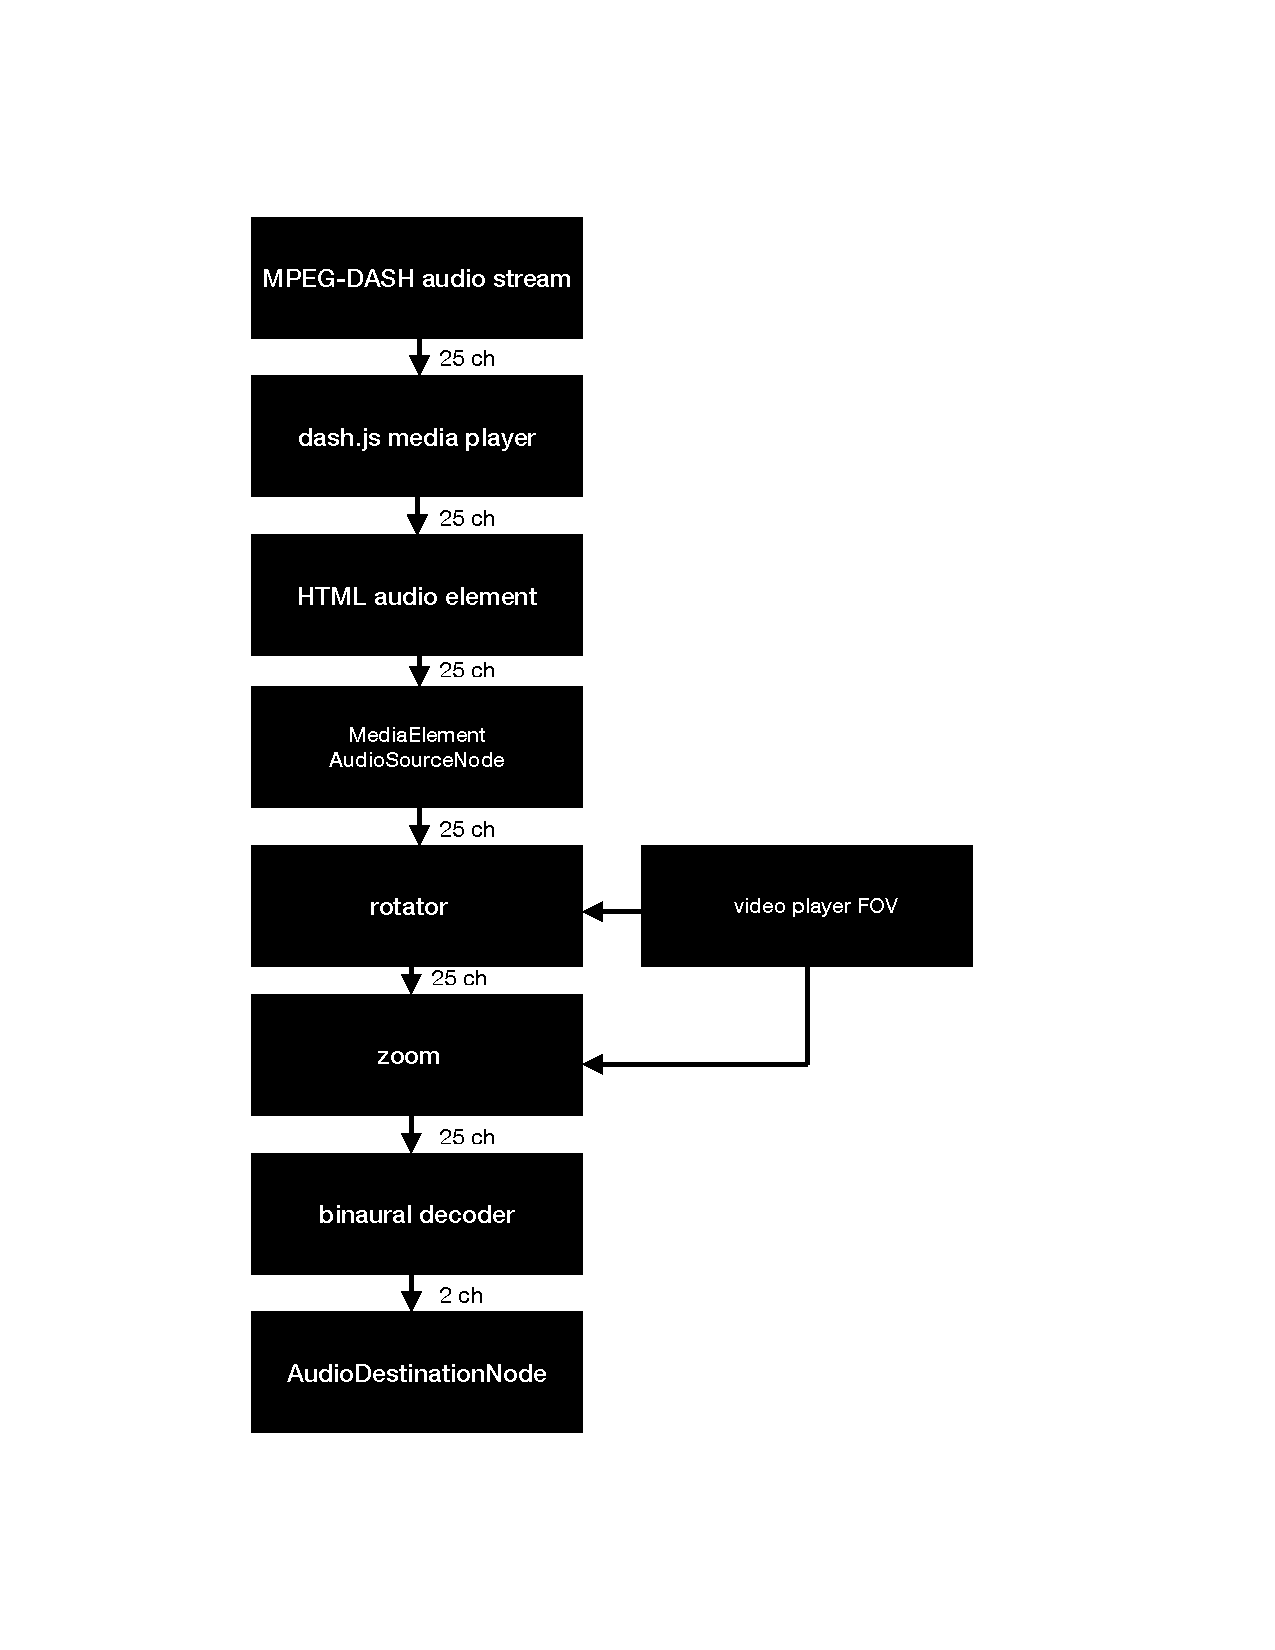
\includegraphics[width=0.9\textwidth]{img/hoast-sig-flow.pdf} 
%\captionsetup{justification=centering}
\caption{HOAST Signal Flow}
\label{fig:hoast-sig-flow}
\end{figure}

Ambisonic zoom is outside the scope of what we wish to cover here, but details about it can be found in the Appendix \ref{ch:appendix-math} under Section \ref{sec:ambi-zoom}. In the next paragraphs we will continue discussing the decoding scheme used, video rendering, and website implementation of HOAST.

\subparagraph{Binaural Decoding}

The \textit{binaural decoding} implemented in HOAST does not involve the traditional \textit{virtual loudspeaker} approach\footnote{As a reminder: in the virtual loudspeaker system, linear combinations of ambisonic harmonics are used to create speaker feeds, identically to ambisonic decoding. The resulting feeds are convolved with HRTFs in the direction of the virtual speaker.}. Instead, the HOAST binaural decoder are based on the solution to a \textit{Least Squares} (LS) problem which results in decoding filters. Deppisch et al. provide the following equation:

\begin{equation}
\omega_{\mathrm{LS}}=\arg \min _{\omega}\left\|\boldsymbol{Y}_{\Upsilon} \boldsymbol{\omega}-\boldsymbol{h}_{\Upsilon}\right\|_{2}^{2}
\label{eq:ls-bin-dec}
\end{equation}

The $(N+1)^2$ decoding filters\footnote{Recall that $N$ refers to the ambisonic order. So we will have a single filter for each ambisonic harmonic.} $\omega_{\mathrm{LS}}$ will minimize the least squares error between HRTF measurements in $\boldsymbol{h}_{\Upsilon}$ and the spherical harmonics in $\boldsymbol{Y}_{\Upsilon}$ evaluated at all HRTF directions in the measurement grid $\Upsilon$ \cite{deppisch2020hoast}. In this case a Lebedev grid\footnote{See appendix} of HRTF measurements is used, and in order to improve the perceptual decoding of binaural signals, the magnitude least squares (MagLS) approach is used. For low frequencies, a LS solution is applied. For reference Equation \ref{eq:arg-min} shows the definition of the $\arg \min$ operator. 

\begin{equation}
\underset{x \in S}{\arg \min } f(x):=\{x \in S: f(s) \geq f(x) \text { for all } s \in S\}
\label{eq:arg-min}
\end{equation}

are points $x$ for which $f(x)$ attains its smallest value. The L2 norm, also used Equation \ref{eq:ls-bin-dec}, is defined as:

\begin{equation}
\|\boldsymbol{x}\|_{2}:=\sqrt{x_{1}^{2}+\cdots+x_{n}^{2}}
\end{equation}

The original set used to generate these filters had $P=2702$ HRTF measurements. The goal of this algorithm is to reduce this to 25 filters for the left ear, and 25 filters for the right (4OA). This is similar to the Resonance architecture \cite{gorzel2019efficient} which accomplishes significant reduction of data using an equivalent approach. A common use of the pseudo-inverse is to computer the LS solution to a system of linear equations. Schorkhuber et al. \cite{schorkhuber2018binaural} discusses in greater detail optimizations to the LS approach to binaural rendering. 

In addition to this LS optimization, the authors also describe the use of a FOA impulse response, generated using the Image Source Method (ISM), in order to improve externalization. This ISM impulse response is applied only to the first-order\footnote{W, Y, Z, X harmonics in ACN ordering, namely.} decoding filters to reduce latency. The length of the higher-order decoding filters is 256 samples. The ISM is a technique that can be used to generate synthetic room impulse responses \cite{allen1979image}\footnote{Detailed discussion of this technique is outside the scope of this chapter.}. 

\subparagraph{Video Rendering}

In order to display 360\textdegree video along with the ambisonic audio, Video.js was used in combination with the videojs-contrib-dash plug-in \cite{deppisch2020hoast}. This allowed the authors to receive and play back MPEG-DASH audio/video streams while supporting equirectangular video\footnote{Equirectangular projection is a typical transform used to display 360 degree content in 2D.} via a custom made plug-in called videojs-xr, which is an update to the pre-existing videojs-vr relying on the newer WebXR API. A polyfill\footnote{Polyfill is a library that: injects an XR implementation into a browser if one does not exist, patches browsers that have incomplete implementations of the API, and, provides a synthesized VR display when WebXR is not supported.} makes HMDs usable in Firefox and Chromium-based browsers. In Chromium-based browsers enabling the \textit{\#webxr} flag, setting the \textit{\#webxr-runtime} and disabling \textit{\#xr-sandbox} might be required.

\subparagraph{Website Implementation}

On the backend side the HOAST web application allows basic CRUD (Create, Read, Update, Delete) tasks of the data. The database holds two main types of data: the meta data of the media files, and, the information related to the "channel" owner (ie. IEM channel). The python-based web framework Django was used, while for the front end the Bootstrap toolkit was used. Currently\footnote{Written in March 2021.} only the creators are allowed to manage the data but the code is freely available so anyone is capable of loading it unto a new server to start their own library. One could also add a more complex backend allowing any user to create their own "channel", but this has not yet been implemented.

% https://immersive-web.github.io/webxr-samples/explainer.html

%https://www.khronos.org/gltf/

% Most usage of WebGL today happens via frameworks that significantly simplify the creation of 3D scenes compared to using raw WebGL. Some of the more popular examples are three.js, babylon.js, and PlayCanvas. There's also frameworks that are specifically designed to create XR content on the web, such as A-Frame and ReactVR. These are all fantastic libraries with their own strengths and focuses, and in general it's recommended that you find tools that suit your needs and rely on them rather than trying to build your own rendering systems from scratch.

% However, most frameworks will also hide away the details of interacting with the WebXR API. That's generally great for users, but not terribly useful when the entire point of your code is to demonstrate how to use the API! At the same time, we don't want the WebXR logic to be obscured by hundreds of lines of WebGL calls. As a result, these samples make use of their own minimalistic rendering library that is specifically designed to highlight use of the WebXR API and de-emphasize the WebGL rendering logic. It is not recommended that you use this library in your own projects, as you will almost certainly be better served by one of the more popular, better established frameworks.

\todo[inline]{Simultaneous Localization and Mapping (SLAM), 360 cameras, matched zone, locomotion}


\section{Open XR Tools}

\section{The Philosophy of "Public Domain"}

\todo[inline]{might move this section to earlier part.}

% Given our focus on the use of FOSS. 

Technology has been an important part of art-making for many decades now. With the decreasing cost of computers, and their improved potential, more people today are capable of making art with computers than ever before. The technology industry remains focused on: improving, updating, and refining its products; in order to generate profit. Unfortunately, these systems are often designed with the latest hardware and operating systems in mind, which places an economic burden on composers and musicians. Furthermore, many popular exhibits and artistic works today feature technology as a core feature of the material, which excludes those who lack access or the skills to create such content.

Software, like digital art, poses a complex economic problem. Unlike physical objects, or direct services, software and digital art can easily be duplicated at little to no cost. Intellectual Property (IP) lies at the heart of this problem as was addressed by Puckette in \cite{puckette2004owns}. In his paper, Puckette used Pure Data (Pd) as a case study of what happens when a research institution commercializes its research. In the article, Puckette argues that IRCAM's\footnote{Institut de Recherche et Coordination Acoustique/Musique.} decision to enforce its IP claims to Pd and sell it as MAX/MSP resulted in a noted drop in the credibility of the institution as a research facility. The name Pd also means Public Domain. Drawing these IP lines is anything but simple since most valuable research draws from other authors' work. Similarly, most worthwhile artworks draw inspiration from its predecessors or contemporaries.

Much like software, digital art can be difficult to price. A physical painting can be analyzed to its authenticity and a price can be set based on what the market is willing to pay for it. A digital sound file, on the other hand, can be duplicated nearly for free, and mass distribution is just as cheap. A musical score operates on basically the same principle. \cite{puckette2001new} explored the idea of bringing some seminal computer music works into the public domain by using Pd, however, not all the works are included on his website, because IRCAM insisted some of patches be taken down. This creates an interesting dilemma for the composers, who naturally would prefer their music be performed as often as possible. 

When working in the scientific domain, one of the applied principles for validating experiments is the reproduction of the research. One of the benefits of using public domain tools, like Pd, is the ability to exercise a similar principle in the artistic domain. The idea being that aesthetic musical principles are hard to extend if the technology inherent to them is proprietary. In the pedagogical domain, this idea is also extremely powerful. Using public domain tools enables one to share their teachings with a wider subset of the population, without having to consider the economic barriers that software can sometimes create. 

Fernando Lopez-Lezcano, a composer and computer scientist at Stanford, has also been interested in this dichotomy for a long time. Fernando has been building Linux distributions for sound research at CCRMA for many years now. In \cite{CEC-eCon28-online} Fernando talks about the traditions established at Stanford related to open source software and how these have evolved over the years. 

%https://econtact.ca/11_3/index.html
%https://econtact.ca/11_3/lopez_lezcano_ccrma.html

\section{The Future of XR}
\section{Conclusion}
